\Section{Network Setup}

Let's briefly summarize the content of the previous chapters. In chapter \ref{ch:theory} the Standard Model of Particle Phyiscs has been presented. It is a remarkable theory explaining the dynamics of elementary particles; however, due to its incompleteness, precision measurements are necessary. The extraction of the $ggZH$ process poses as a suitable candidate for such measurements at the CMS experiment, described in chapter \ref{ch:experiment}. In order to achieve that, new analysis techniques based on deep learning (chapter \ref{ch:deeplearning}) are being explored. The exact analysis strategy and -setup has been described in chapter $\ref{ch:analysis_strategy}$.

In this chapter the cINN setup which will be used for inferring the signal strength modifiers $\mu_i$ will be discussed. In the first half, the generation of the training and test datasets with a detailed focus on the analysis specifics, such as interpolation between histograms (morphing) and the representation of the statistic and systematic uncertainties is going to be elaborated.

In the second half of this chapter, the final cINN architecture is going to be presented. The inference results and the interpretation of the network outputs will be discussed in the next chapter.

\Subsection{Training Dataset Generation}

The conditions shown in fig \ref{fig:conditions} in chapter \ref{ch:analysis_strategy} represent the expectation on the measured dataset. Unfortunately, the exact share of each signal process in each bin in the measured data is a priori unknown (which would mean the complete physics is known to the very last detail). For this purpose the different scenarios of a signal process having more or less shares in a bin have to be first artificially represented in the dataset in order to obtain a cINN which is capable of inferring the share of each signal process -- or in other words, to obtain the signal modifier parameters $\mu_i$. For this, both signal and background processes have to be scaled to achieve the desired sensitivity towards different scenarios.

\Subsubsection{Prior Selection}

In order to do so, a set of signal modifier parameters are drawn from a pool of expected parameter distribution (the prior). Then, each process in the histogram is scaled with the corresponding parameter and the bins will summed up meaning (similar to the expected dataset) the information about the exact contribution of each process to each bin is lost thereafter.

The prior distribution for the processes have been selected as the following. For the signal processes \texttt{ggZH}, \texttt{ZHDY} and \texttt{WH} the $\mu_i$ were sampled from a gamma distribution

\begin{equation*}
	\Gamma(x; k, \theta) = \frac{x^{k-1}e^{-x/\theta}}{\theta^k\Gamma(k)}
\end{equation*}

with shape parameter $k$, scale $\theta$ and $\Gamma(k)$ being the gamma function. An advantage of this distribution as prior is the positiveness of the samples $\{x_i\}$ from the distribution as negative signal modifier parameters carry no physical meaning; apart from that, the distribution has a long tail for increasing values of $x$ which allow a more fined selection in a given range while maintaining some generalization property. The parameters were set to be $k = 1.5$ and $\theta = 7$; with this specific selection, one obtains a prior which is sensitive in the low signal yield region $\mu \lesssim 10$ while maintaining network sensitivity for values $\mu\lesssim100$.

For the background processes, it is expected that the MC simulations follow the expectation with good accuracy. Hence, one expects $\mu \approx 1$. For this reason, the prior has been chosen to follow a lognormal distribution

\begin{equation*}
	\mathcal{N}(x; \mu, \sigma) = \frac{1}{\sqrt{2\pi }\sigma x}\exp\left(-\frac{\left(\ln x-\mu\right)^2}{2\sigma^2}\right)
\end{equation*}

with mean $\mu = 0.05$ and $\sigma = 0.25$, lognormal distributions being positive themselves.

In order the estimate the arising uncertainty from the luminosity, the obtained conditions (after scaling and uncertainty variation) are then scaled with an additional luminosity factor. These have been drawn from a lognormal distribution with $\mu = 0$ and $\sigma = 0.02$. All distributions are shown in fig. \ref{fig:priors}.

With these priors, the cINN has a total of 17 inputs for 3 signal, 13 background modifier parameters and the luminosity nuisance parameter.

\begin{figure}[h!]
	\centering
	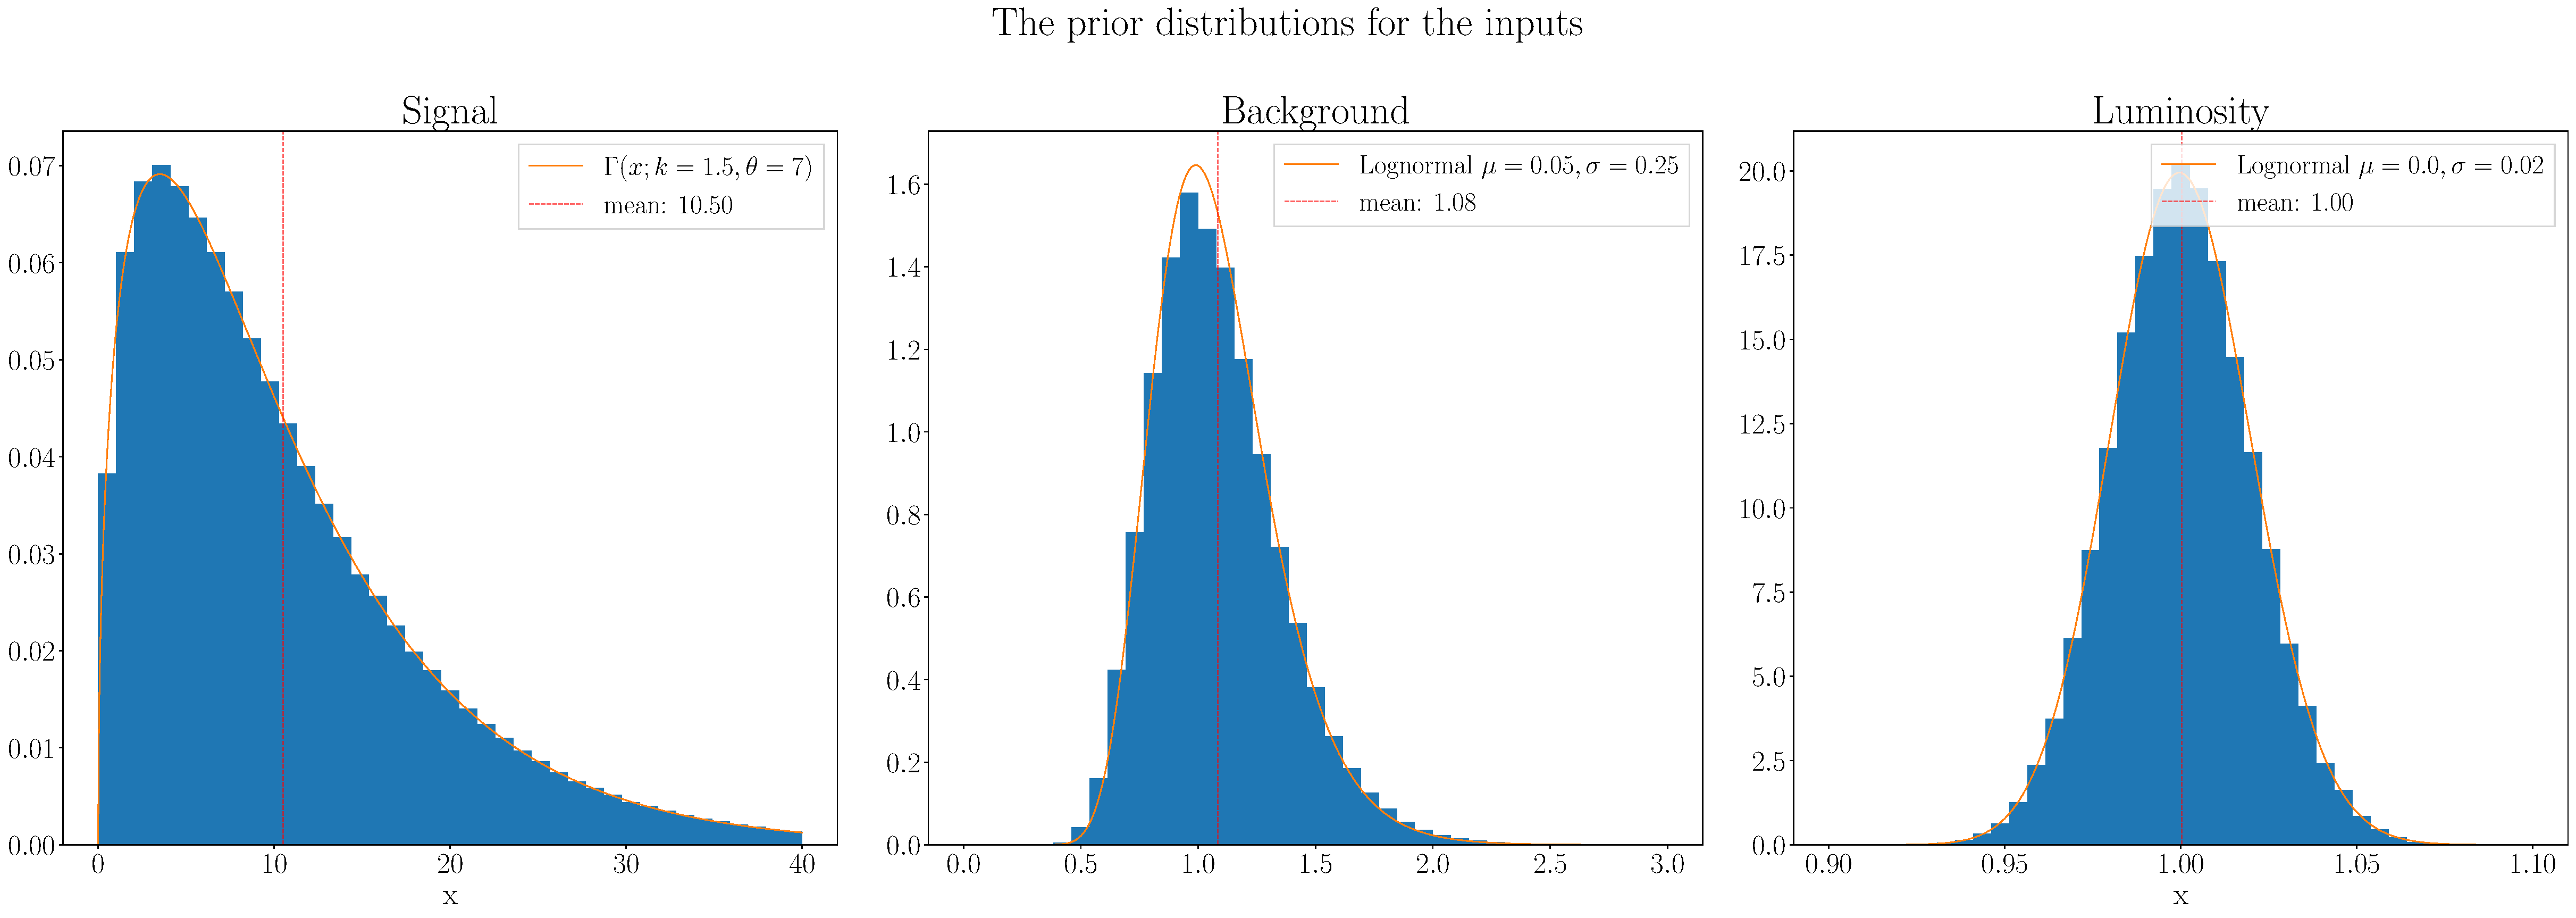
\includegraphics[width=\linewidth]{figures/network_setup/priors.pdf}
%	\begin{minipage}{.5\textwidth}
%		\centering
%%		\includegraphics[width=0.8\linewidth]{figures/network/signal}
%	\end{minipage}%
%	\begin{minipage}{.5\textwidth}
%		\centering
%%		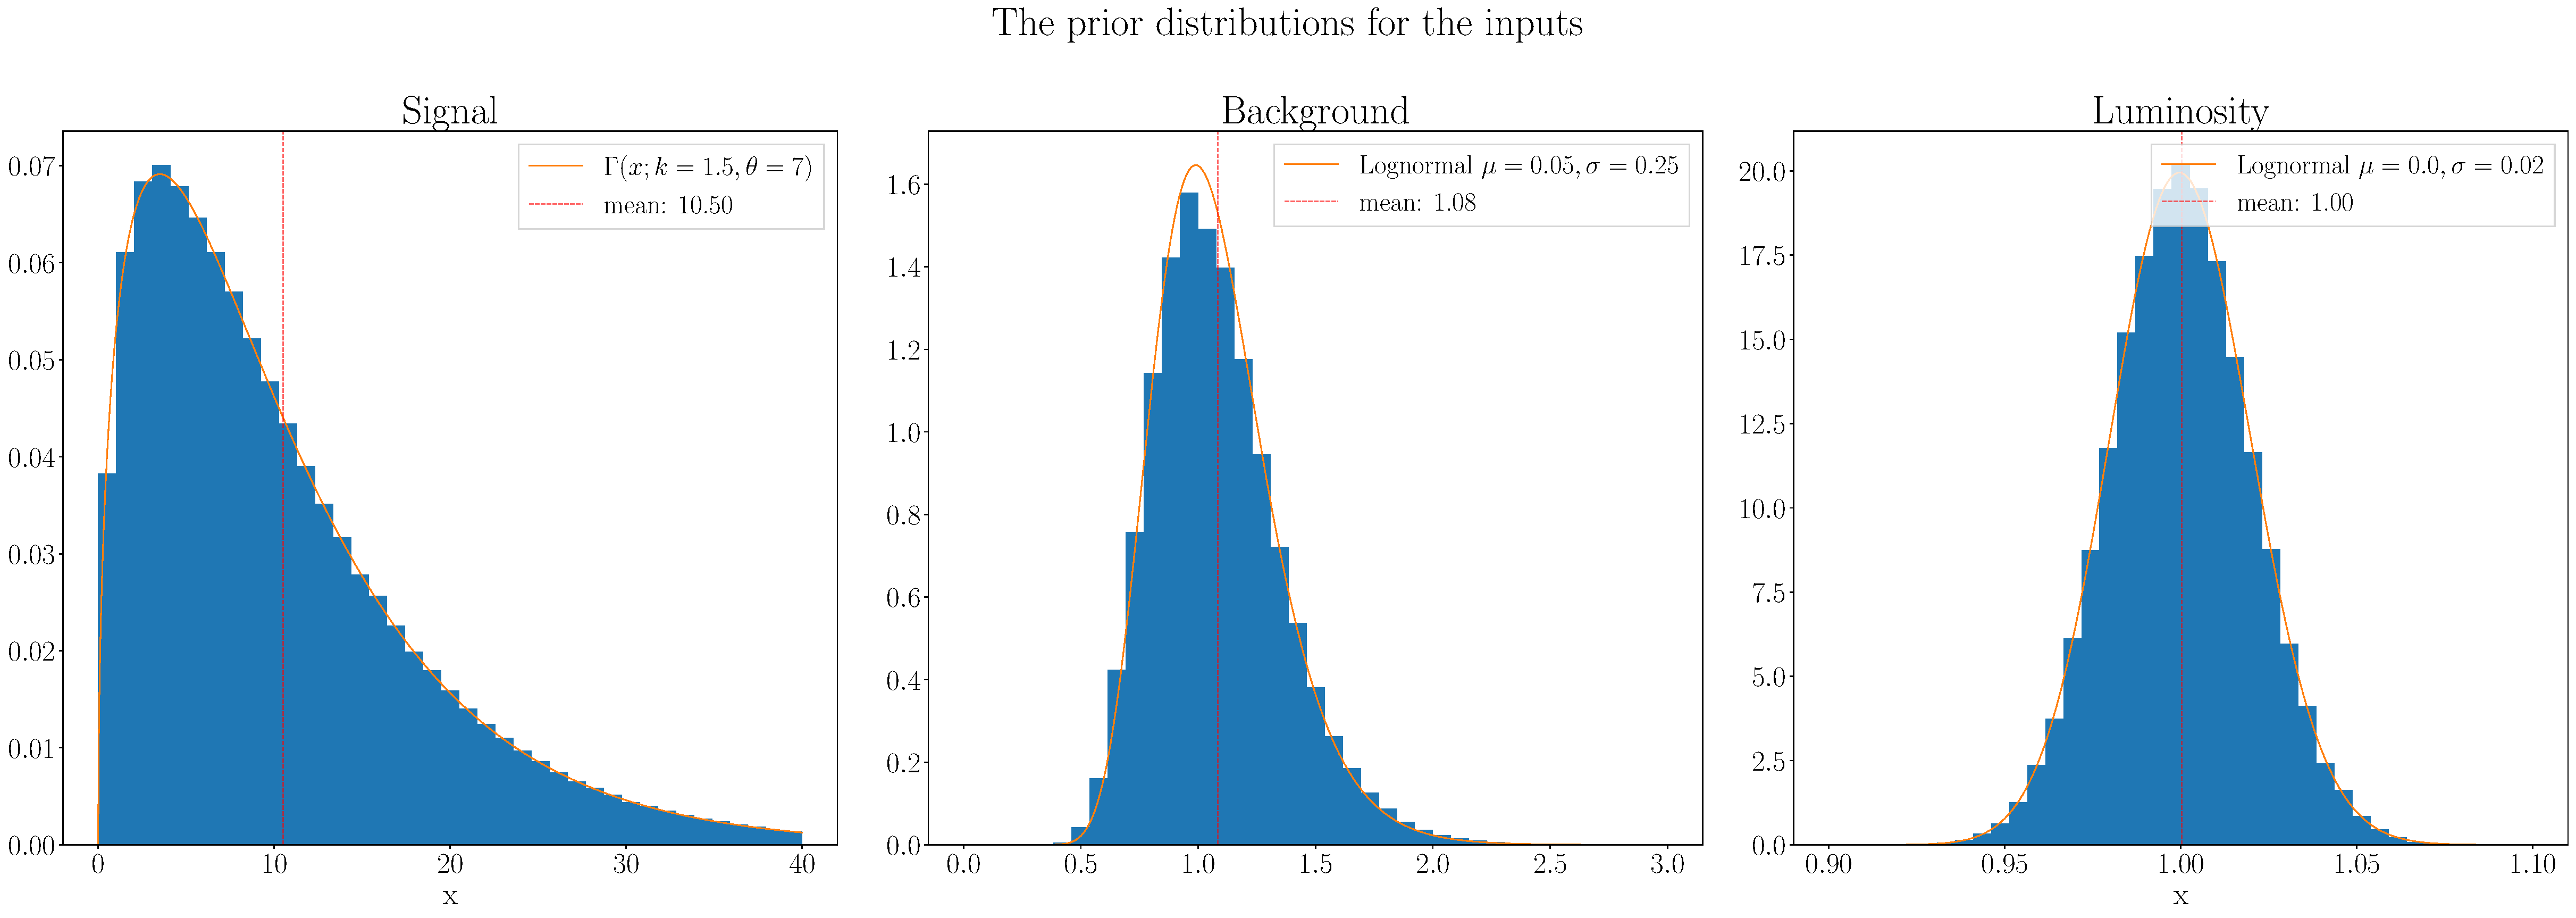
\includegraphics[width=0.6\linewidth]{figures/network_setup/priors.pdf}
%	\end{minipage}
	\caption{Prior distributions for the signal and background processes. Samples are shown in blue; the mean of each distribution is shown with the red dashed line. The analytic shape of each distribution is shown in orange.}
	\label{fig:priors}
\end{figure}

It does not suffice to scale the processes with their respective parameters exclusively, as systematic and statistic effects change the overall shape of the resulting histogram. For this reason, the nuisance parameter effects have to be mapped onto the training and test dataset in order to avoid that the network learns features not present in a general measured dataset.

\Subsubsection{Systematic Uncertainties}

The systematic uncertainties require an interpolation method as the shifts in the histograms are computationally expensive to obtain. In other words, as only the effect of the $1\sigma$ up- and down-shifts of the uncertainties (templates) are given, the task is to represent the in-between-cases (and obviously, those on the outside of the given range) in the histrograms. For this purpose, a non-linear histogram morphing method has been implemented.

In the following, an overview on the treated uncertainties and the morphing algorithm will be given with a discussion on the implementation and on its effects on the histograms following thereafter.

\Subsubsection{Normalization and Shape-Changing Uncertainties}

There are 25 nuisance parameter which have been taken into account. These can be grouped into normalization and shape-changing uncertainties.

Normalization uncertainties do not affect the shape of the histograms. Rather, they have an equal effect on each bin (hence the name "normalization"). To this group belong the following: the luminosity uncertainty and the parton density function uncertainity (which arise from the unknown interaction initial state due to the nontrivial proton structure).

The shape-changing uncertainties influence all histogram bins differently and incorporate most uncertainties in this work. The 23 shape-changing and the parton density function normalization uncertainties have been listed in tab. \ref{tab:s_sys_table}; interpolation among these systematic effects given the $1\sigma$ shifted histograms have been performed via histogram morphing, which will be discussed in the next section. In order to study the network's nuisance parameter expressive power, the luminosity uncertainty has been treated as an input.

\begin{table}[h!]
	\centering
	\begin{tabular}{cc}
		Uncertainty name               & Description \\
		
		\hline
		\texttt{PDFSet} & Parton density function uncertainty \\
		
		\hline
		$\begin{aligned}
			\texttt{PSWeight}&\texttt{\_FSR} & \\
			\texttt{PSWeight}&\texttt{\_ISR} & \\
		\end{aligned}$ & $\begin{array}{c}
			\text{Parton shower mismodelling uncertainties} \\
			\text{for final and initial state radiation}
		\end{array}$ \\
		
		\hline
		$\begin{aligned}	
			\texttt{ScaleWeight}&\texttt{\_Envelope} \\
			\texttt{ScaleWeight}&\texttt{\_Fact    } \\
			\texttt{ScaleWeight}&\texttt{\_Mixed   } \\
			\texttt{ScaleWeight}&\texttt{\_Renorm  } \\
		\end{aligned}$ & Jet energy scale uncertainties \\
		
		\hline
		% https://twiki.cern.ch/twiki/bin/viewauth/CMS/BtagRecommendation#preUL_scale_factor_uncertainties
		$\begin{aligned}
			\texttt{btagWeight}&\texttt{\_lf       } \\
			\texttt{btagWeight}&\texttt{\_cferr1   } \\
			\texttt{btagWeight}&\texttt{\_cferr2   } \\
			\texttt{btagWeight}&\texttt{\_hf       } \\
			\texttt{btagWeight}&\texttt{\_hfstats1 } \\
			\texttt{btagWeight}&\texttt{\_hfstats2 } \\
			\texttt{btagWeight}&\texttt{\_lfstats1 } \\
			\texttt{btagWeight}&\texttt{\_lfstats2 } \\
		\end{aligned}$ & b-tag score weight correction uncertainties \\
		
		\hline
		\texttt{l1\_ecal\_prefiring  } & 2017 ECAL miss-calibration correction uncertainty \\
		
		\hline		
		% https://twiki.cern.ch/twiki/bin/view/CMS/MuonReferenceEffs2017
		$\begin{aligned}
			\texttt{electron}&\texttt{\_reco } \\
			\texttt{electron}&\texttt{\_id   } \\
			\texttt{muon}&\texttt{\_id       } \\
			\texttt{muon}&\texttt{\_iso      } \\
		\end{aligned}$         & $\begin{array}{c}
			\text{Lepton identification, reconstruction} \\
			\text{and isolation uncertainties}
		\end{array}$\\
		
		\hline
		$\begin{aligned}
			\texttt{trigger}&\texttt{\_ee\_sf  } \\
			\texttt{trigger}&\texttt{\_mu\_sf  } \\
			\texttt{trigger}&\texttt{\_mumu\_sf} \\
		\end{aligned}$ & Trigger efficiency uncertainties \\
		\hline
		% https://twiki.cern.ch/twiki/bin/view/CMS/PileupSystematicErrors
		\texttt{pileup               } & Pileup uncertainty \\
	\end{tabular}
	\caption{The morphed one normalization (\texttt{PDFSet}) and the other 23 shape-changing uncertainties with a brief description.}
	\label{tab:s_sys_table}
\end{table}

\Subsubsection{Non-Linear Histogram Morphing}

Non-linear histogram morphing has been implemented on the basis of \cite{Baak_2015}. For the interpolation a nominal distribution and -- in this case -- 24 other distribution templates representing the $1\sigma$ and $-1\sigma$ shifts are given. The nominal template $f(x|m)$ with morphing parameter $m$ can then be approximated around $m=0$ with the other templates in a simple 1D case using

\begin{equation*}
	f(x|m) \approx \sum_j \left.\frac{\partial^{(j)} f(x|m)}{\partial m^{(j)}}\right|_{m=0}\frac{m^j}{j!} = \sum_j f_j'(x|m=0) m^j
\end{equation*}



where the derivatives and the factorials have been absorbed in $f'_j$.

For $T$ uncorrelated uncertainties (hence for $T$ morphing parameters $m$) with morphing parameter values $\pm1$ there are $2T+1$ sampled distributions in total (counting the nominal distribution, defined as $m=0$). An intuitive representation of the "morphing parameter space" with the indication of the available templates is shown in fig. \ref{fig:morphing_phase_space}.

\begin{figure}[h!]
	\centering
	\centering
	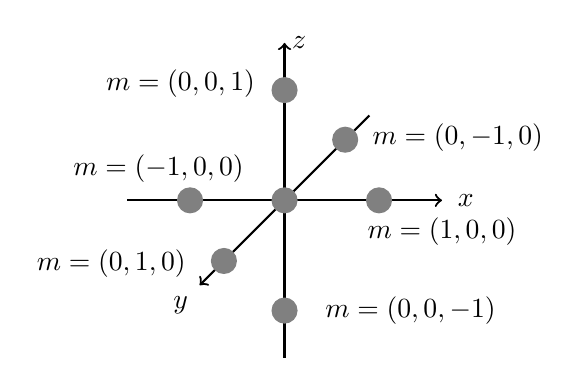
\begin{tikzpicture}[scale=2]
		\coordinate (O) at (0,0,0);
		\draw[thick,->] (-1.,0,0) -- (1.,0,0) node[right=2]{$x$};
		\draw[thick,->] (0,-1,0) -- (0,1,0) node[right=-1]{$z$};
		\draw[thick,->] (0,0,-1.4) -- (0,0,1.4) node[below left=0.5]{$y$};
		
		\node[circle, fill=gray] (0) {};
		\node[circle, fill=gray] at (   0,-0.7, 0) {};
		\node at (0.8, -0.7, 0) {$m=(0,0,-1)$};
		\node[circle, fill=gray] at (   0, 0.7, 0) {};
		\node at (-1.2, 0.2, -1.4) {$m=(0,0,1)$};
		\node[circle, fill=gray] at (   0, 0  ,-1) {};
		\node at (-0.8, 0.2, 0) {$m=(-1,0,0)$};
		\node[circle, fill=gray] at (   0, 0  , 1) {};
		\node at (1, -0.2, 0) {$m=(1,0,0)$};
		\node[circle, fill=gray] at (-0.6, 0  , 0) {};
		\node at (-1.1, -0.4, 0) {$m=(0,1,0)$};
		\node[circle, fill=gray] at ( 0.6, 0  , 0) {};
		\node at (1.1, 0.4, 0) {$m=(0,-1,0)$};
	\end{tikzpicture}
	\caption{The morphing "phase space" showing the available distributions for $T=3$ uncertainties of $\sigma=\pm1$. The available templates in the phase space are shown in grey. Note that the nominal template with $m=(0,0,0)$ lies in the origin and there are no "mixed" templates (such as $m = (1,1,0)$) available. In the setting described above, one has $T=24$, hence there are $24\times2 +1 = 49$ templates in total.}
	\label{fig:morphing_phase_space}
\end{figure}

For this multidimensional case where there are no "mixed templates" as the above uncertainties are considered to be uncorrelated. Hence, the mixed derivative terms from the above expansion are zero and the expression can be written for a given $\mathbf{m}_i$\footnote{$\mathbf{m}_i = (0, 0, ..., 0, \pm 1, 0, ..., 0)$ for the i-th template with $\sigma=\pm1$} as:

\begin{equation}
	f(x | \mathbf{m}_i) = \underbrace{\vphantom{\frac{1}{2!}\left.\frac{\partial^2 f(x | \mathbf{m})}{\partial m_j^2}\right|_{\mathbf{m}=0}}f(x | 0)}_{f_0} + \sum^T_{j=1} \underbrace{\vphantom{\frac{1}{2!}\left.\frac{\partial^2 f(x | \mathbf{m})}{\partial m_j^2}\right|_{\mathbf{m}=0}}\left.\frac{\partial f(x | \mathbf{m})}{\partial m_j}\right|_{\mathbf{m}=0}}_{f'_j}(m_i)_j + \sum^T_{j=1} \underbrace{\frac{1}{2!}\left.\frac{\partial^2 f(x | \mathbf{m})}{\partial m_j^2}\right|_{\mathbf{m}=0}}_{f'_{jj}}(m_i)^2_j + \mathcal{O}\left((m_i)_j^3\right)
	\label{eq:morphing}
\end{equation}

where $(m_i)_j$ denotes the j-th component of the i-th morphing parameter vector. The aim is to find an expression for the unknown derivatives as only the histogram $f(x|\mathbf{m})$ (but not its derivative) is given. If one knew the derivatives, one could easily select a general $\mathbf{m}_i$ and insert in into eq. \ref{eq:morphing}, obtaining the morphed distribution.

In order to express the derivatives write all given templates in a vectorized form, and make use of the matrix form

\begin{equation*}
	\left(\begin{aligned}
		f\Bigl(x &| (0,\phantom{-}0, 0\,,...,\phantom{-}0)\Bigl) \\
		f\Bigl(x &| (0,\phantom{-}1, 0\,,...,\phantom{-}0)\Bigl) \\
		f\Bigl(x &| (0,-1, 0\,,...,\phantom{-}0)\Bigl) \\
		&\vdots \\
		f\Bigl(x &| (0,\phantom{-}0, 0\,,...,\phantom{-}1\Bigl) \\
		f\Bigl(x &| (0,\phantom{-}0, 0\,,...,-1\Bigl) \\
	\end{aligned}\right) = \underbrace{\left(\begin{matrix}
		1 & 0 & 0 & 0 & & 0 & 0 \\
		1 & 1 & 1 & 0 &  \cdots & 0 & 0 \\
		1 & -1 & 1 & 0 &      & 0 & 0 \\
		& & \vdots & & \ddots & \vdots & \\
		1 & 0 & 0 & 0 &       & 1 & 1 \\
		1 & 0 & 0 & 0 & \cdots & -1 & 1 \\
	\end{matrix}\right)}_{M} \left(\begin{matrix}
	f_0 \\
	f'_1 \\
	f'_{11} \\
	\vdots \\
	f'_T \\
	f'_{TT}
\end{matrix}\right)
\end{equation*}

With an invertible coefficient matrix $M \in \mathbb{R}^{49\times49}$, encoding the position of the templates in the morphing phase space. Inverting $M$\footnote{Note that thanks to the block matrix structure the inversion is computationally feasible. In addition, the inverse has to be evaluated only once.}

\begin{equation*}
	M^{-1} = \left(\begin{matrix}
		 1 & 0   & 0   & 0 &        & 0 & 0 \\
		 0 & 0.5 &-0.5 & 0 & \cdots & 0 & 0 \\
		-1 & 0.5 &\phantom{-}0.5 & 0 &        & 0 & 0 \\
		   & \vdots &     &    & \ddots &  & \vdots \\
		 0 & 0   & 0   & 0 &        & 0.5 & -0.5 \\
		-1 & 0   & 0   & 0 & \cdots & 0.5 & \phantom{-}0.5 \\
	\end{matrix}\right)
\end{equation*}

this collapses into

\begin{equation*}
	M^{-1}\mathbf{f} = \mathbf{f}'
\end{equation*}

and eq. \ref{eq:morphing} can be then written for a general $\mathbf{m}$ as

\begin{equation}
	f(x|\mathbf{m}) = (1, m_1, m_1^2, ..., m_T, m^2_T) M^{-1}\mathbf{f}
	\label{eq:final_morphing}
\end{equation}

Eq. \ref{eq:final_morphing} is the final shape of the morphing algorithm implemented for the representation of the effect of the 24 nuisance parameters in the dataset. The results of applying morphing for some selected nuisance parameters are discussed in the next chapter.

\Subsubsection{Systematic Uncertainty Representation in Training Data}

The effect of the morphing algorithm from above has been studied by looking at some arbitrary histograms explicitly. Below an example for one normalisation and two shape-changing uncertainties for both morphing parameters $m=-0.5$ and $m = 0.5$ is given.

For the parton desitity function uncertainty, negative values of $m$ decrease the event content of each bin, while $m>0$ yields more events compared to the nominal histogram. As a normalisation uncertainty, it keeps the shape of the distribution. This behaviour can be seen in fig. \ref{fig:pdfset}.

\begin{figure}[h!]
	\centering
	\begin{minipage}{.5\textwidth}
		\centering
		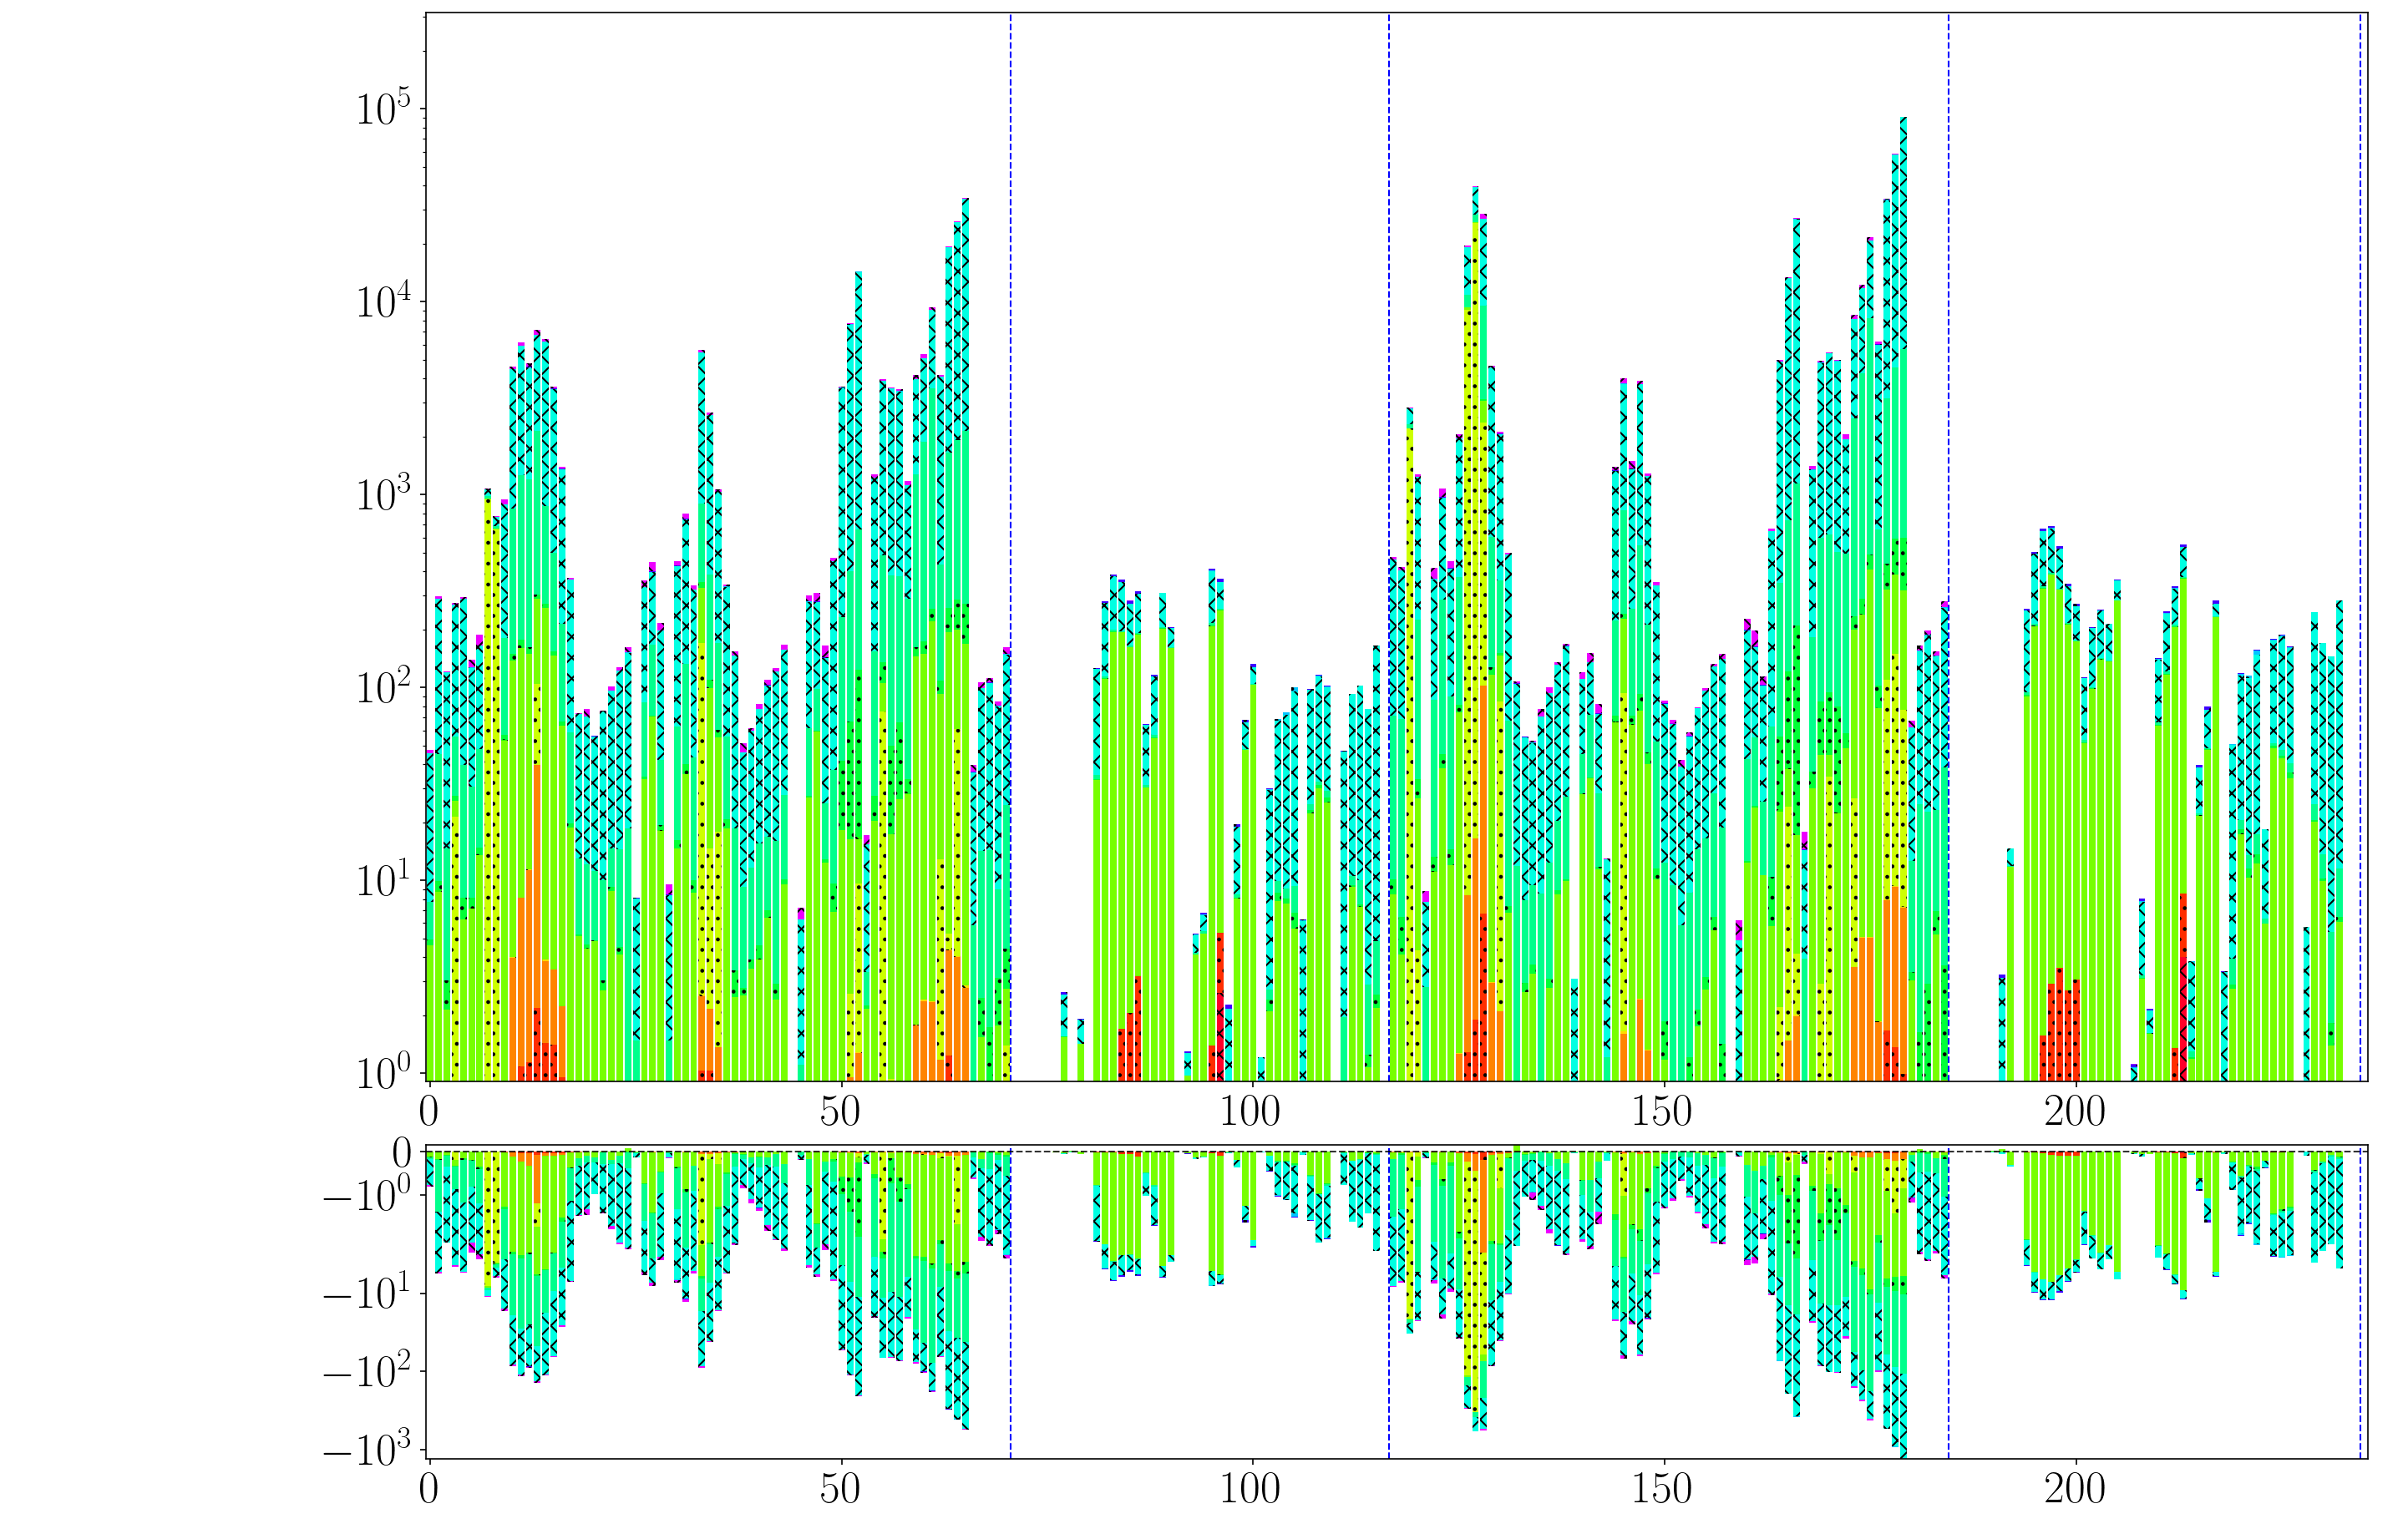
\includegraphics[width=\linewidth]{figures/network_setup/PDFSet_-0.5}
	\end{minipage}%
	\begin{minipage}{.5\textwidth}
		\centering
		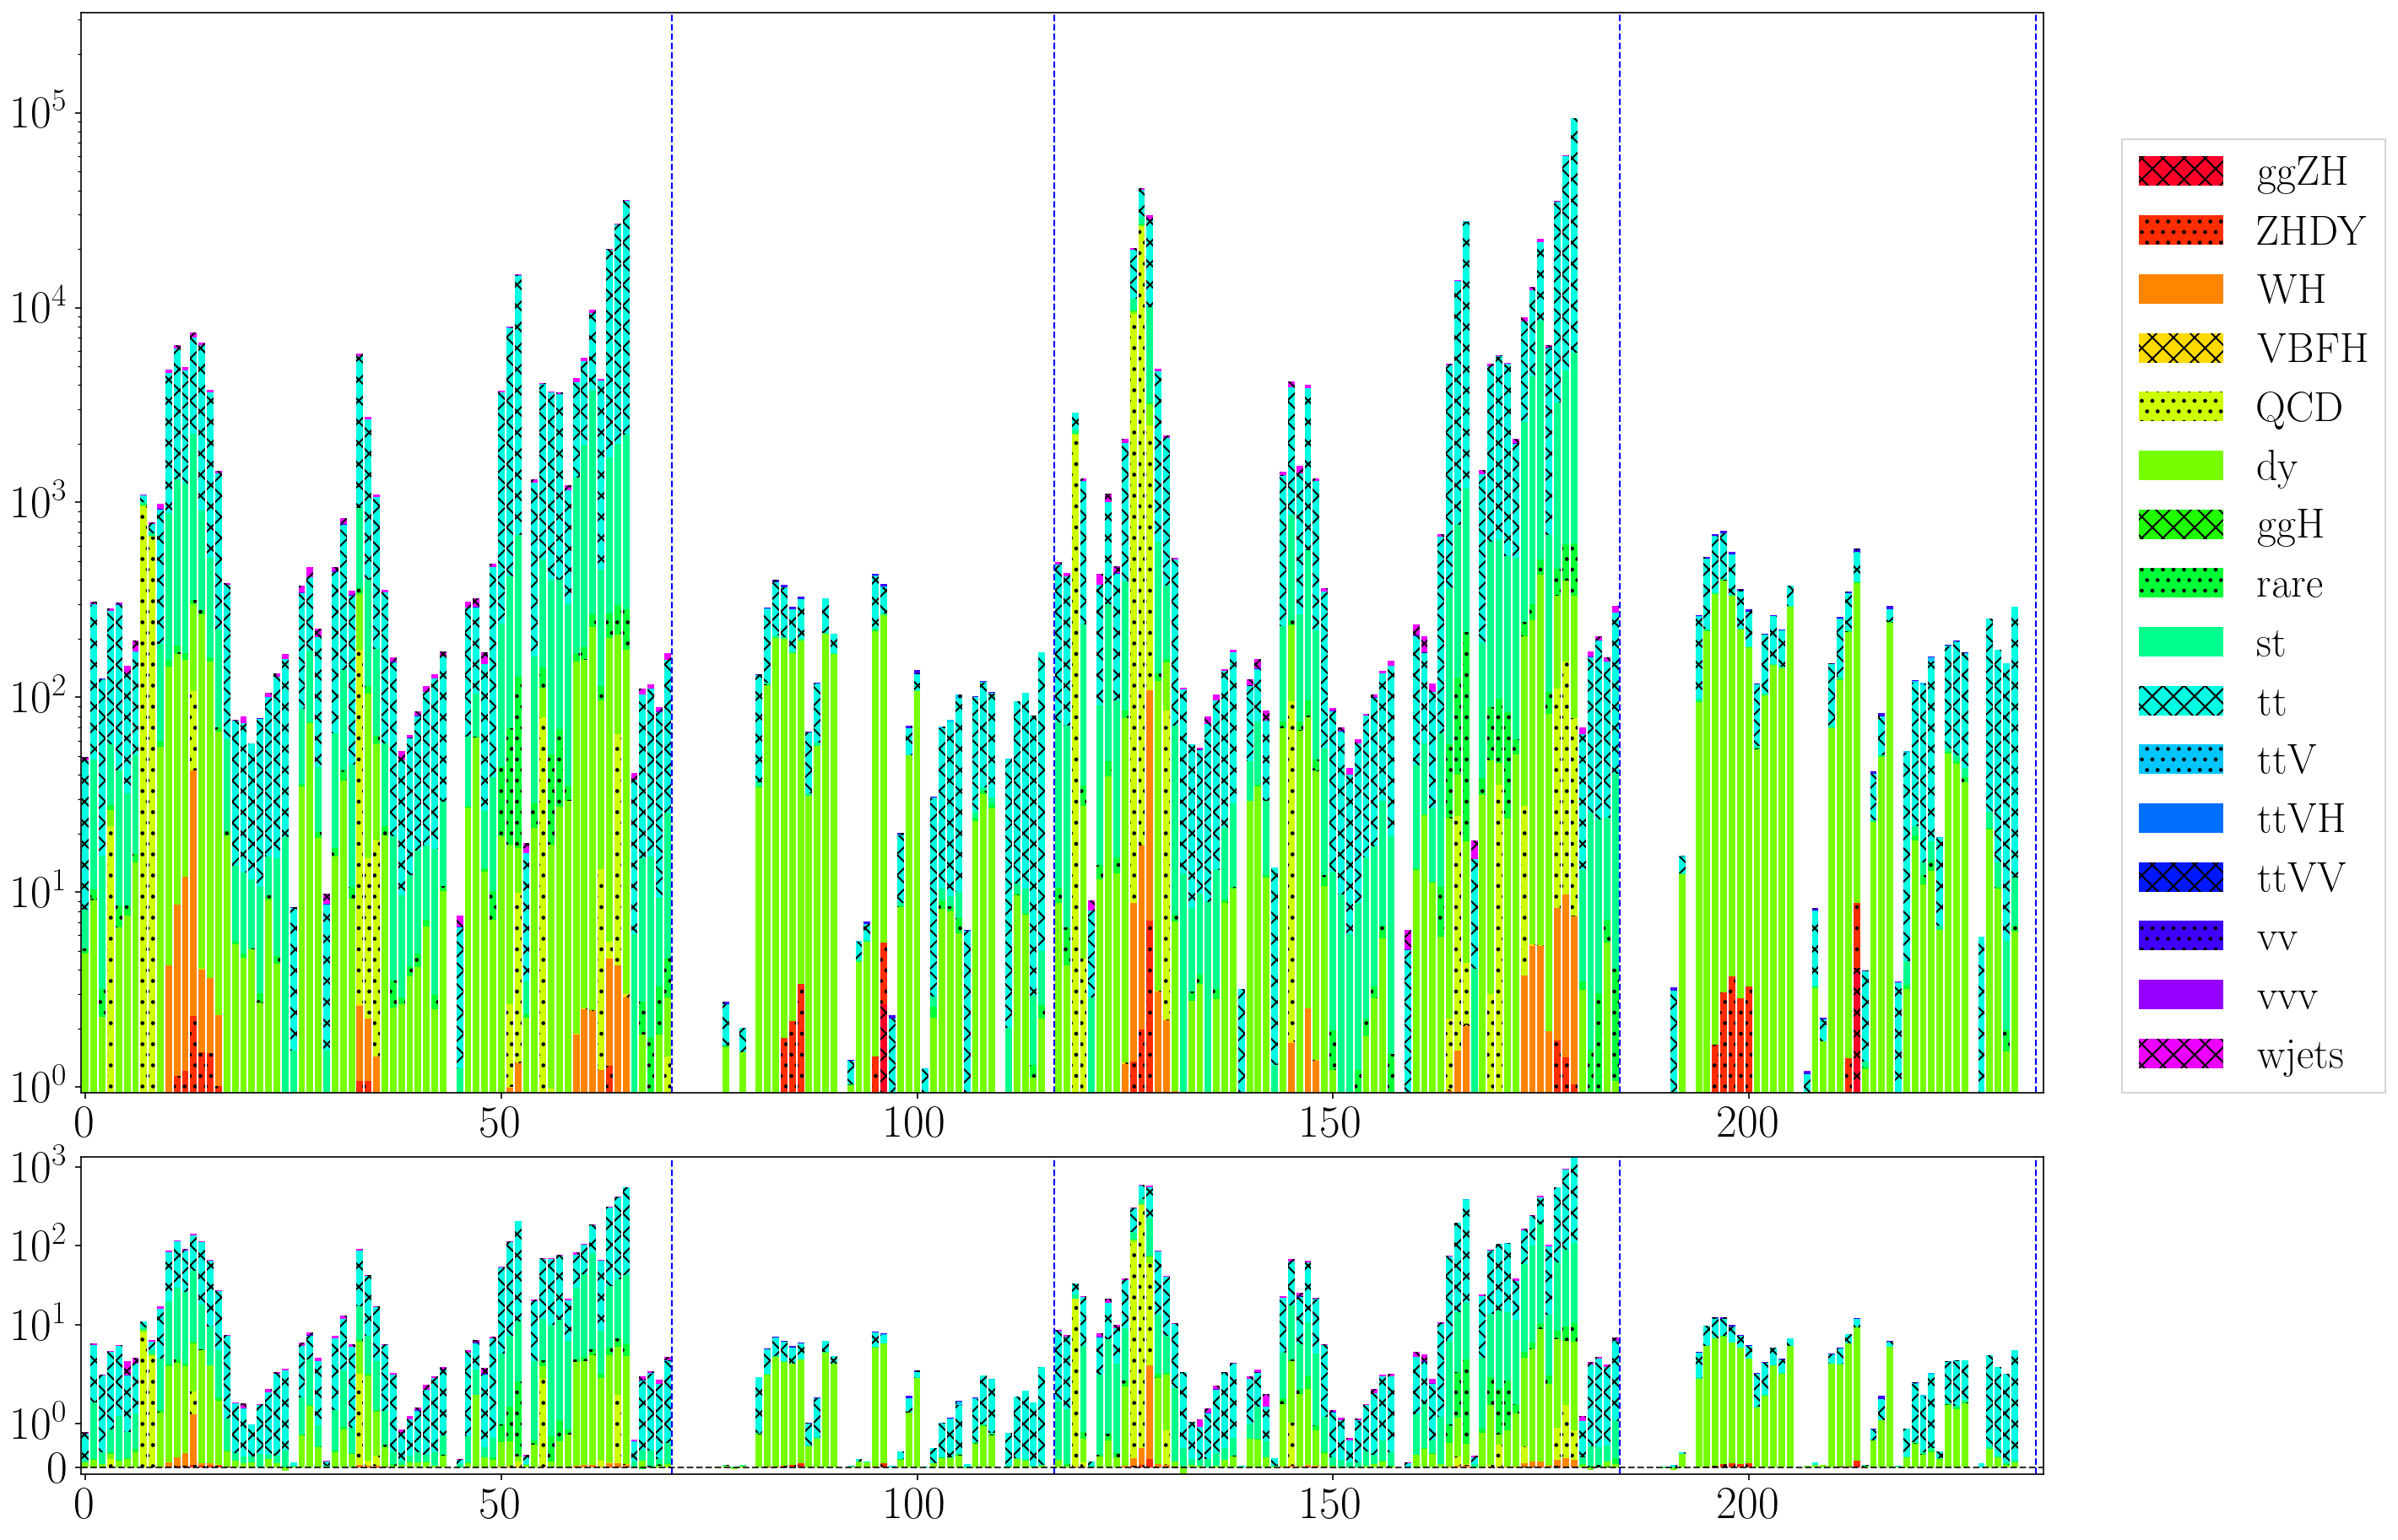
\includegraphics[width=\linewidth]{figures/network_setup/PDFSet_+0.5}
	\end{minipage}
	\caption{Morphed histograms for $m = -0.5$ (left) and $m = +0.5$ (right) for \texttt{PDFSet} for the $e$, $ee$, $\mu$ and $\mu\mu$ categories separated with the blue dashed line. Below the difference of the morphed histogram to the nominal histogram ($m = 0$) is shown. Note that each bin has been influenced uniformly, keeping the overall shape of the conditions.}
	\label{fig:pdfset}
\end{figure}

As a shape-changing uncertainty, $\texttt{pileup}$ influences all bins separately. Due to this behaviour, the content of a given bin for a process might increase in one bin but decrease in another bin for the same morphing parameter. The morphed histogram for the same morphing parameters are shown in fig. \ref{fig:pileup}.

\begin{figure}[h!]
	\centering
		\begin{minipage}{.5\textwidth}
				\centering
				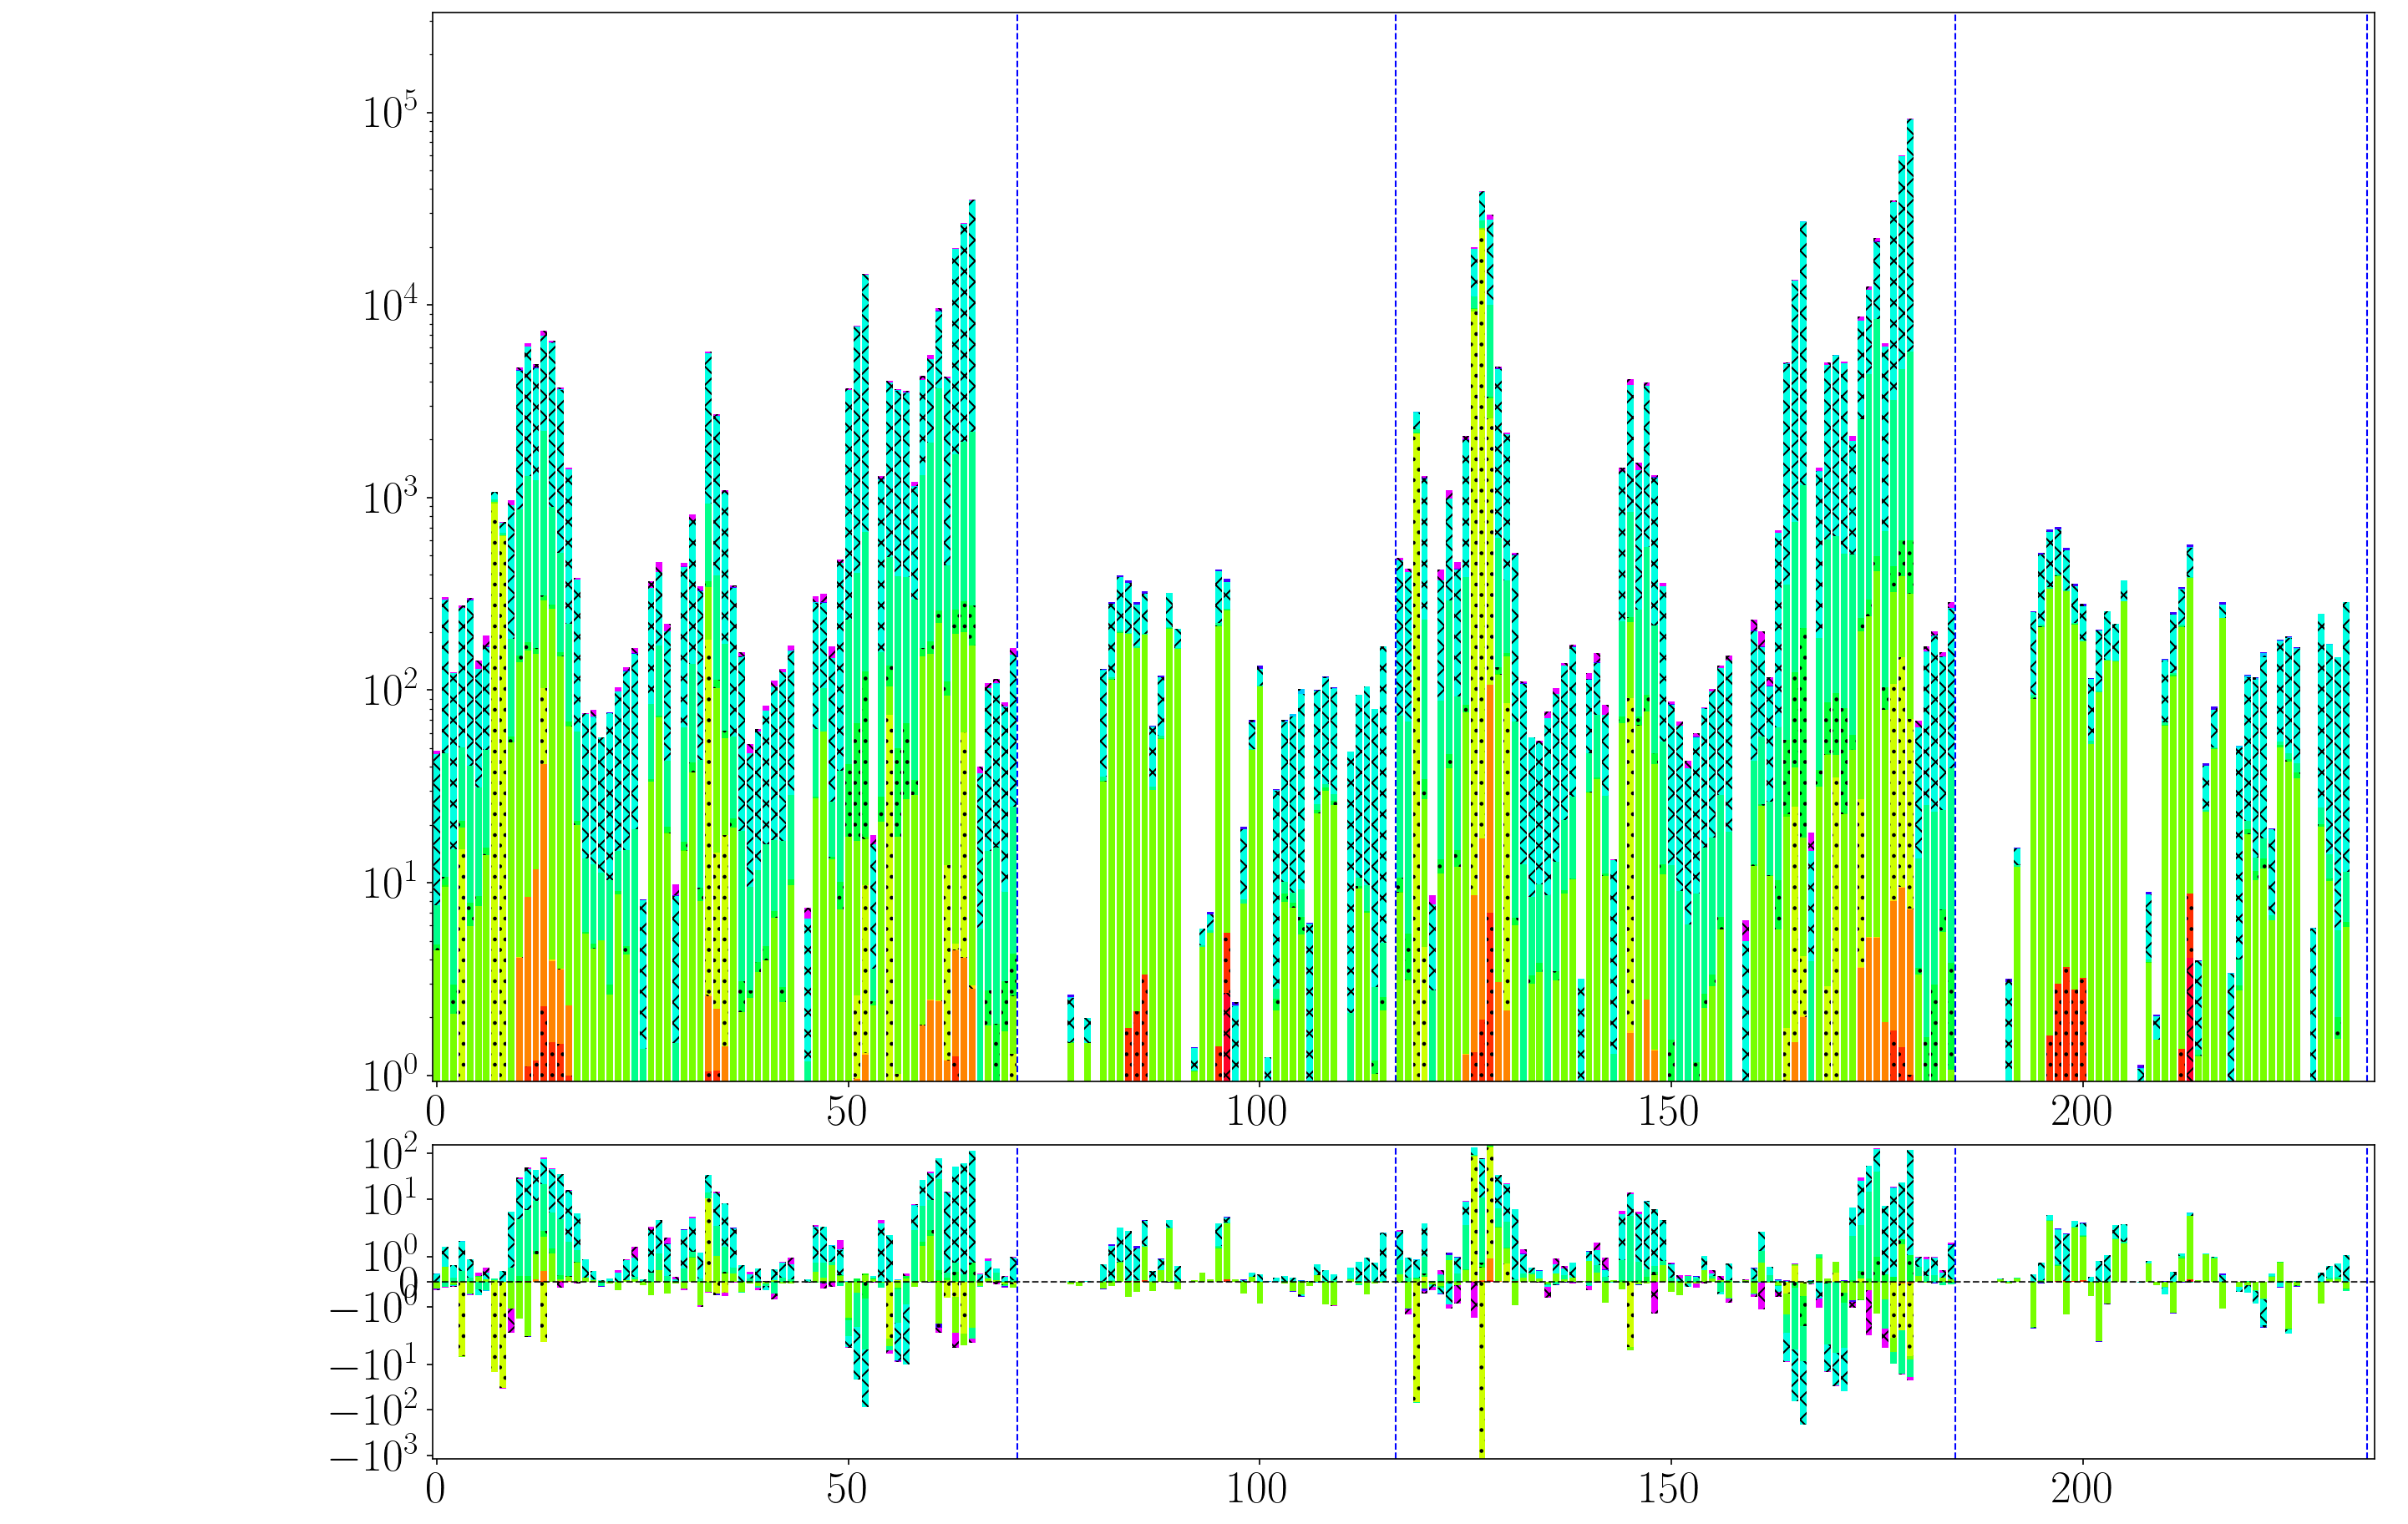
\includegraphics[width=\linewidth]{figures/network_setup/pileup_-0.5}
			\end{minipage}%
		\begin{minipage}{.5\textwidth}
				\centering
				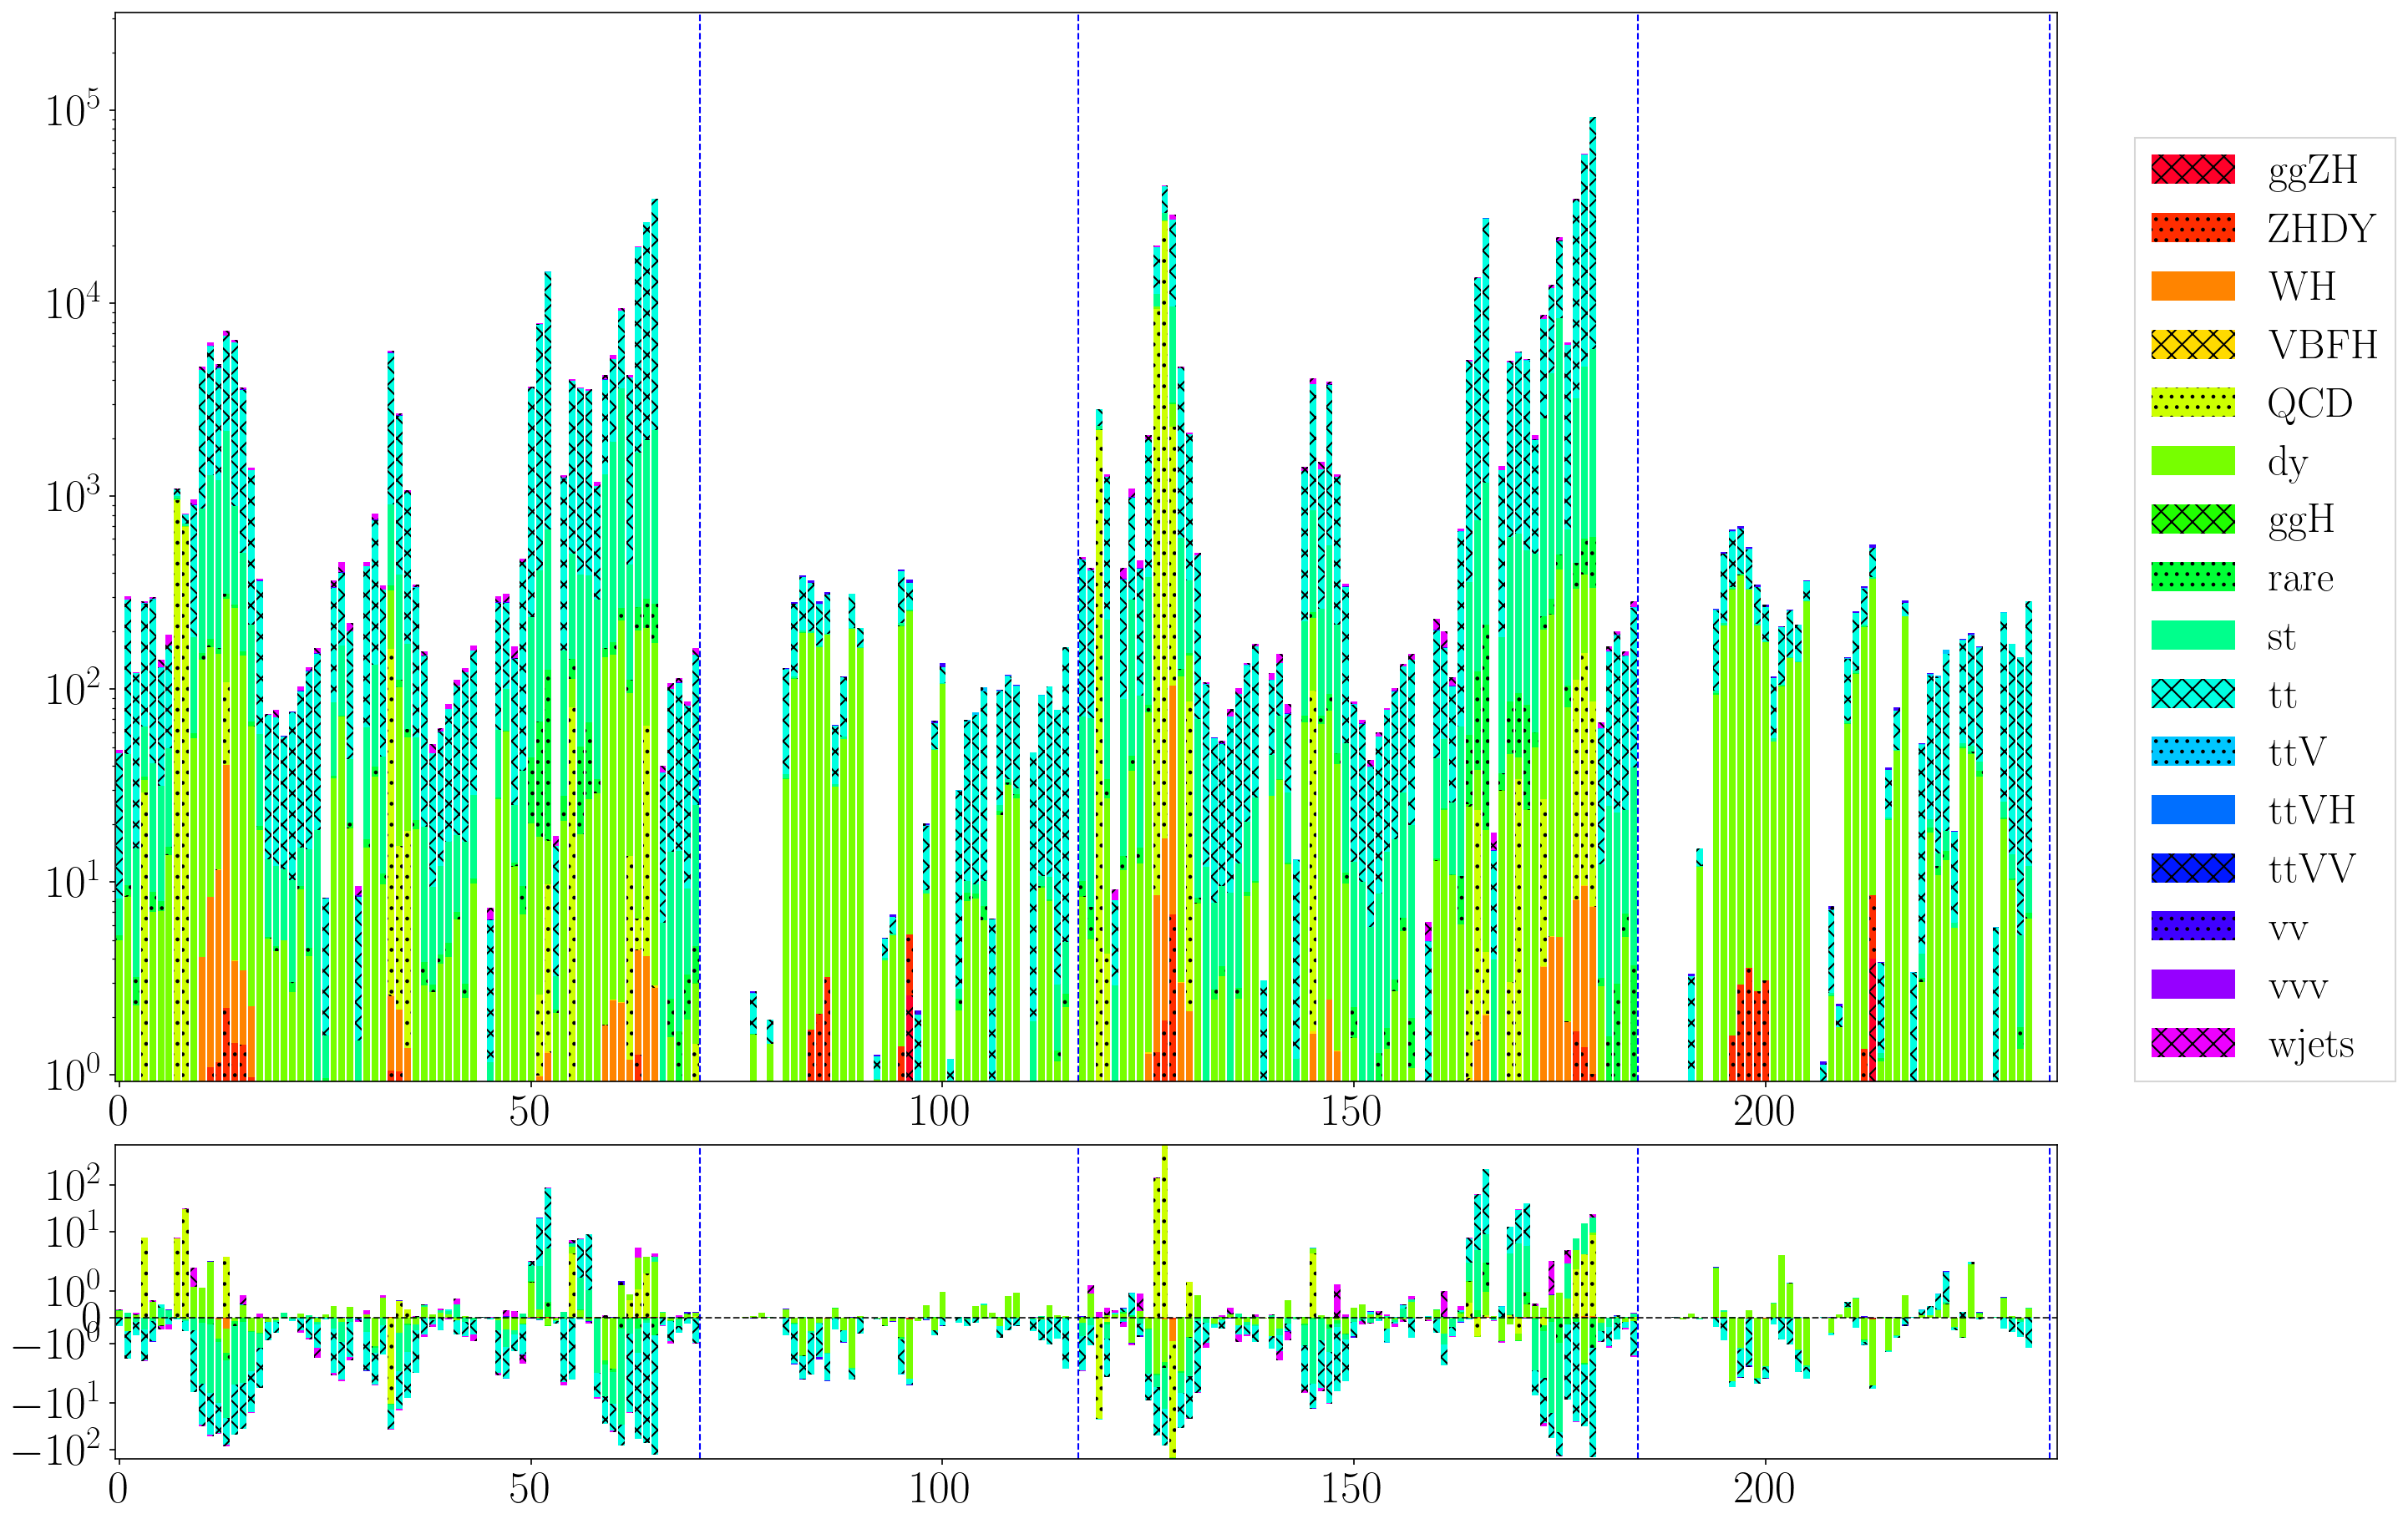
\includegraphics[width=\linewidth]{figures/network_setup/pileup_+0.5}
			\end{minipage}
	\caption{Morphed histograms for $m = -0.5$ (left) and $m = +0.5$ (right) for \texttt{pileup}. Below the difference of the morphed histogram to the nominal histogram is shown. Note that effect is different for each process and in each bin as expected for a shape changing uncertainty.}
	\label{fig:pileup}
\end{figure}

As the second shape-chaning uncertainty to showcase, the dilepton trigger efficiency effects have been chosen. Due to their focus on given $\mu\mu$ or $ee$ final states, these uncertainties influence single categories only. The effect of \texttt{trigger\_mumu\_sf} and \texttt{trigger\_ee\_sf} are shown in fig. \ref{fig:trigger_sf}.

\begin{figure}[h!]
	\centering
	\begin{minipage}{.5\textwidth}
		\centering
		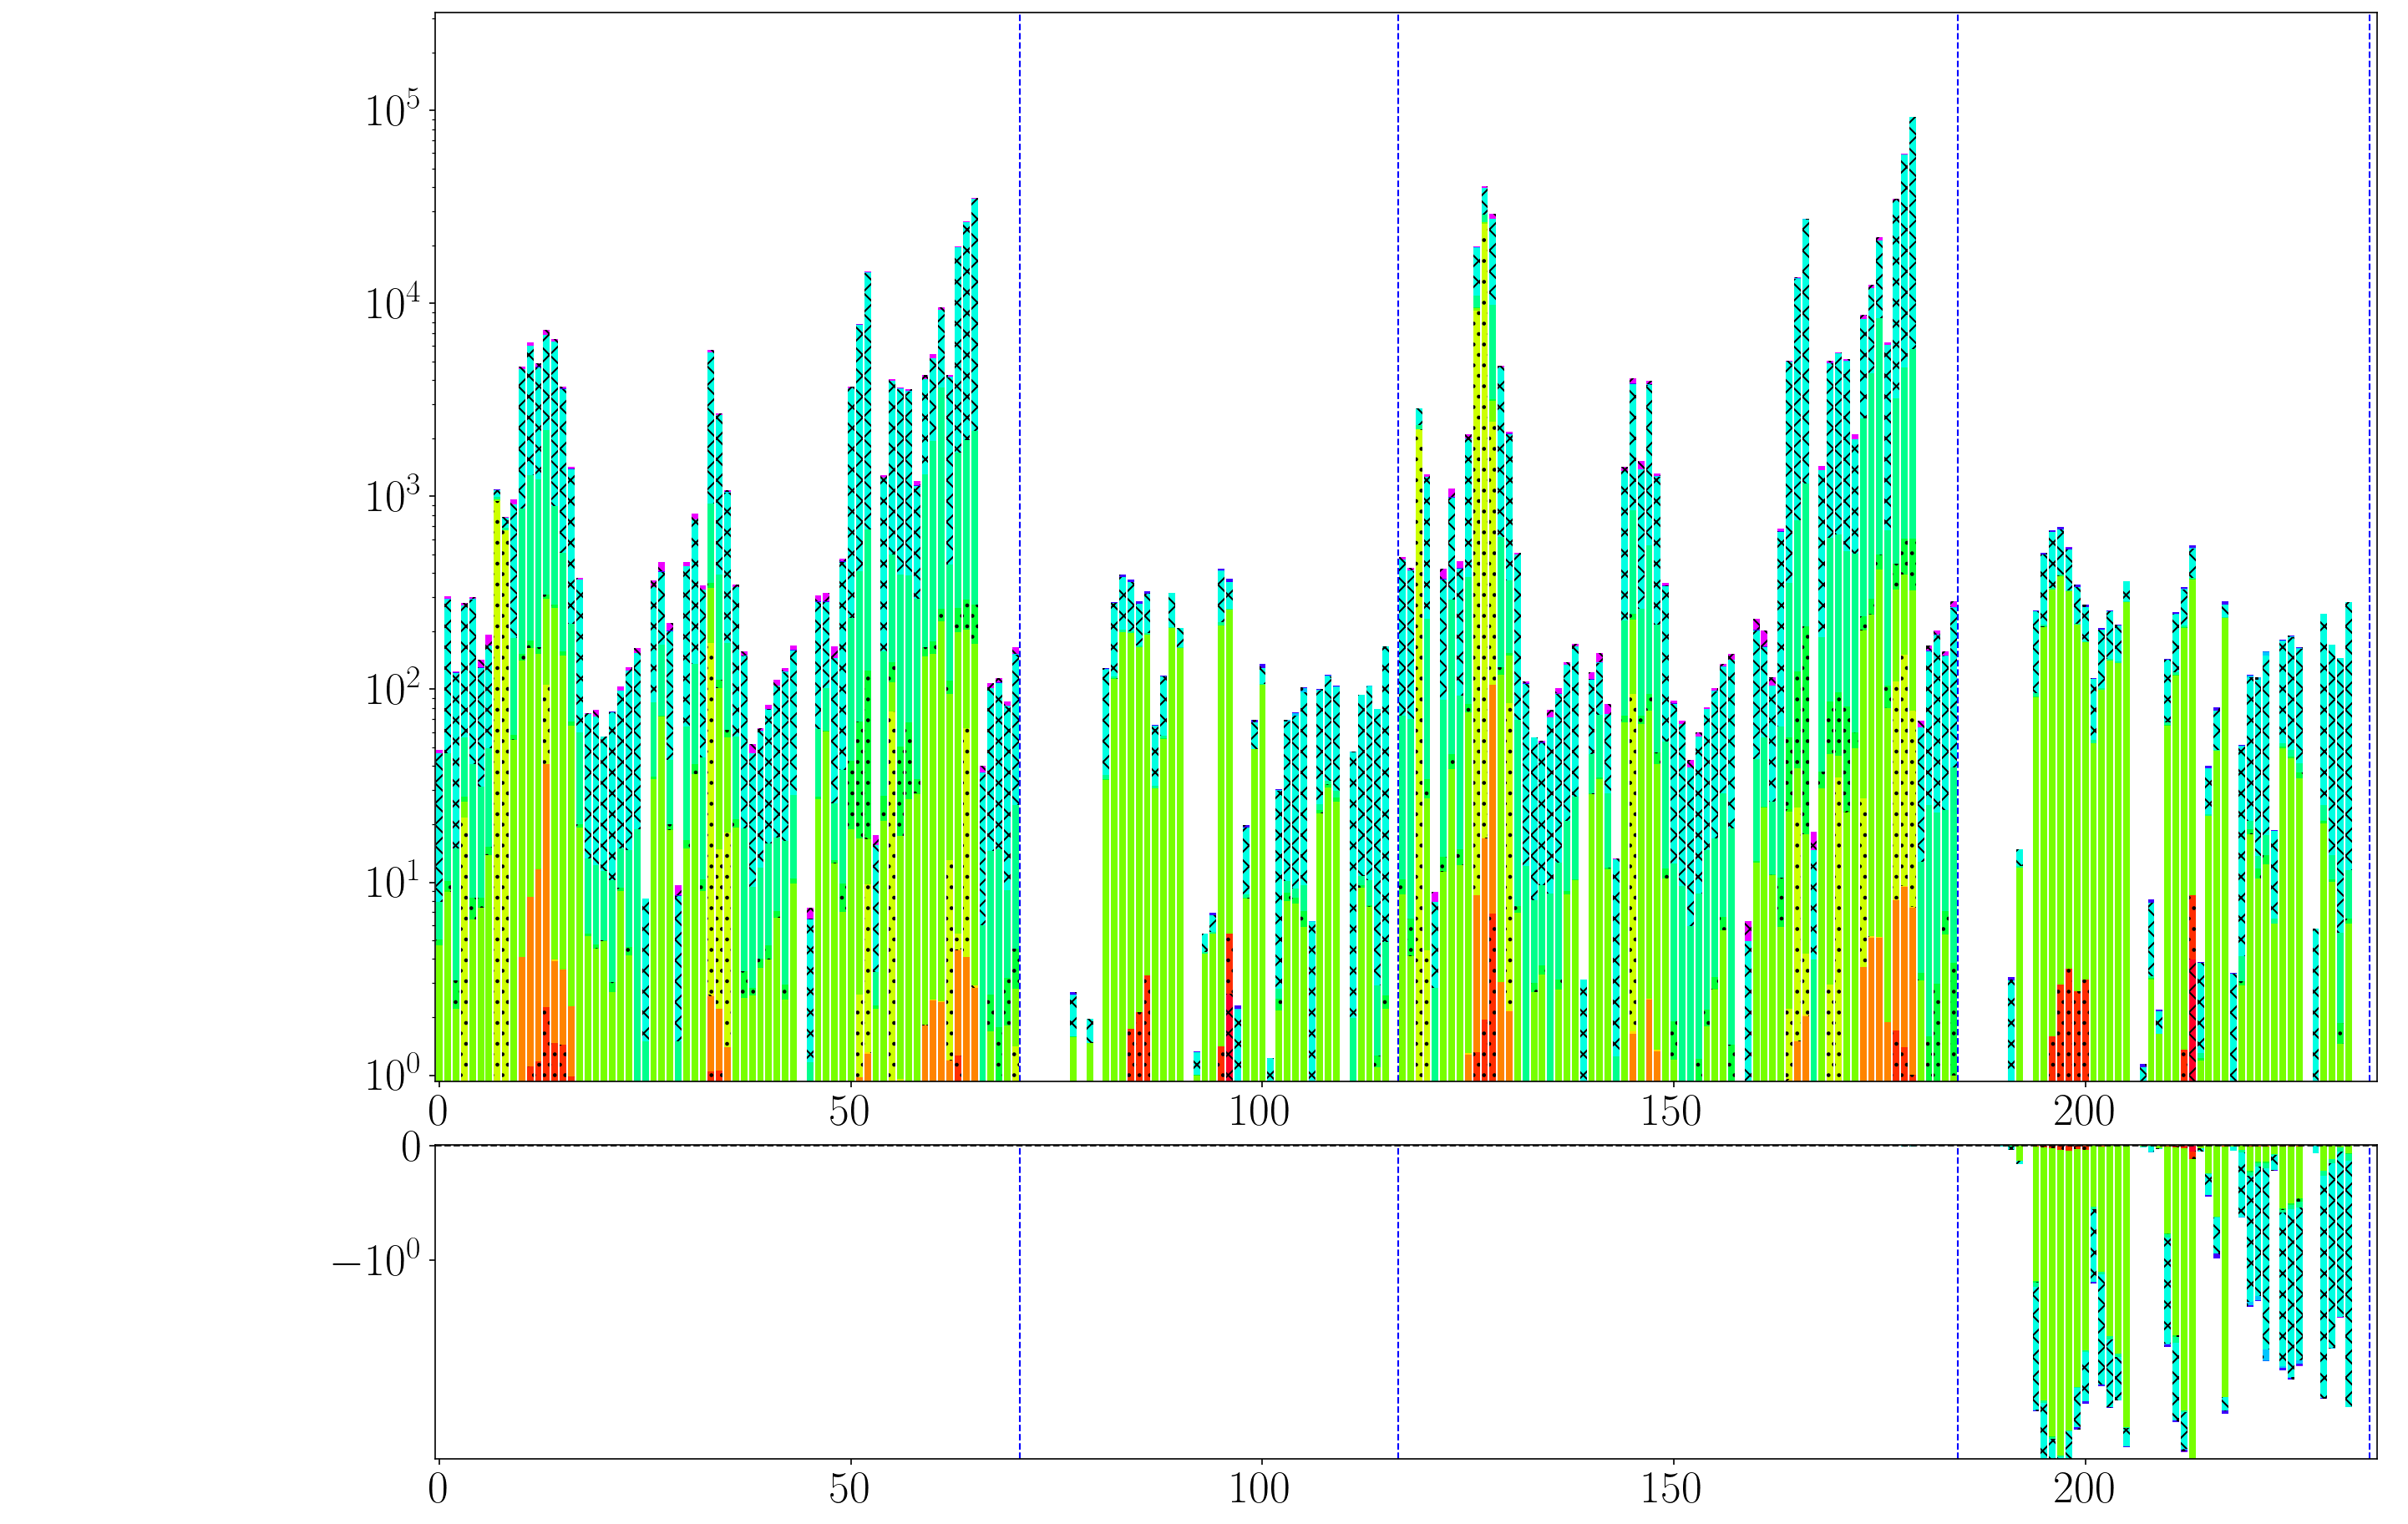
\includegraphics[width=\linewidth]{figures/network_setup/trigger_mumu_sf_-0.5}
		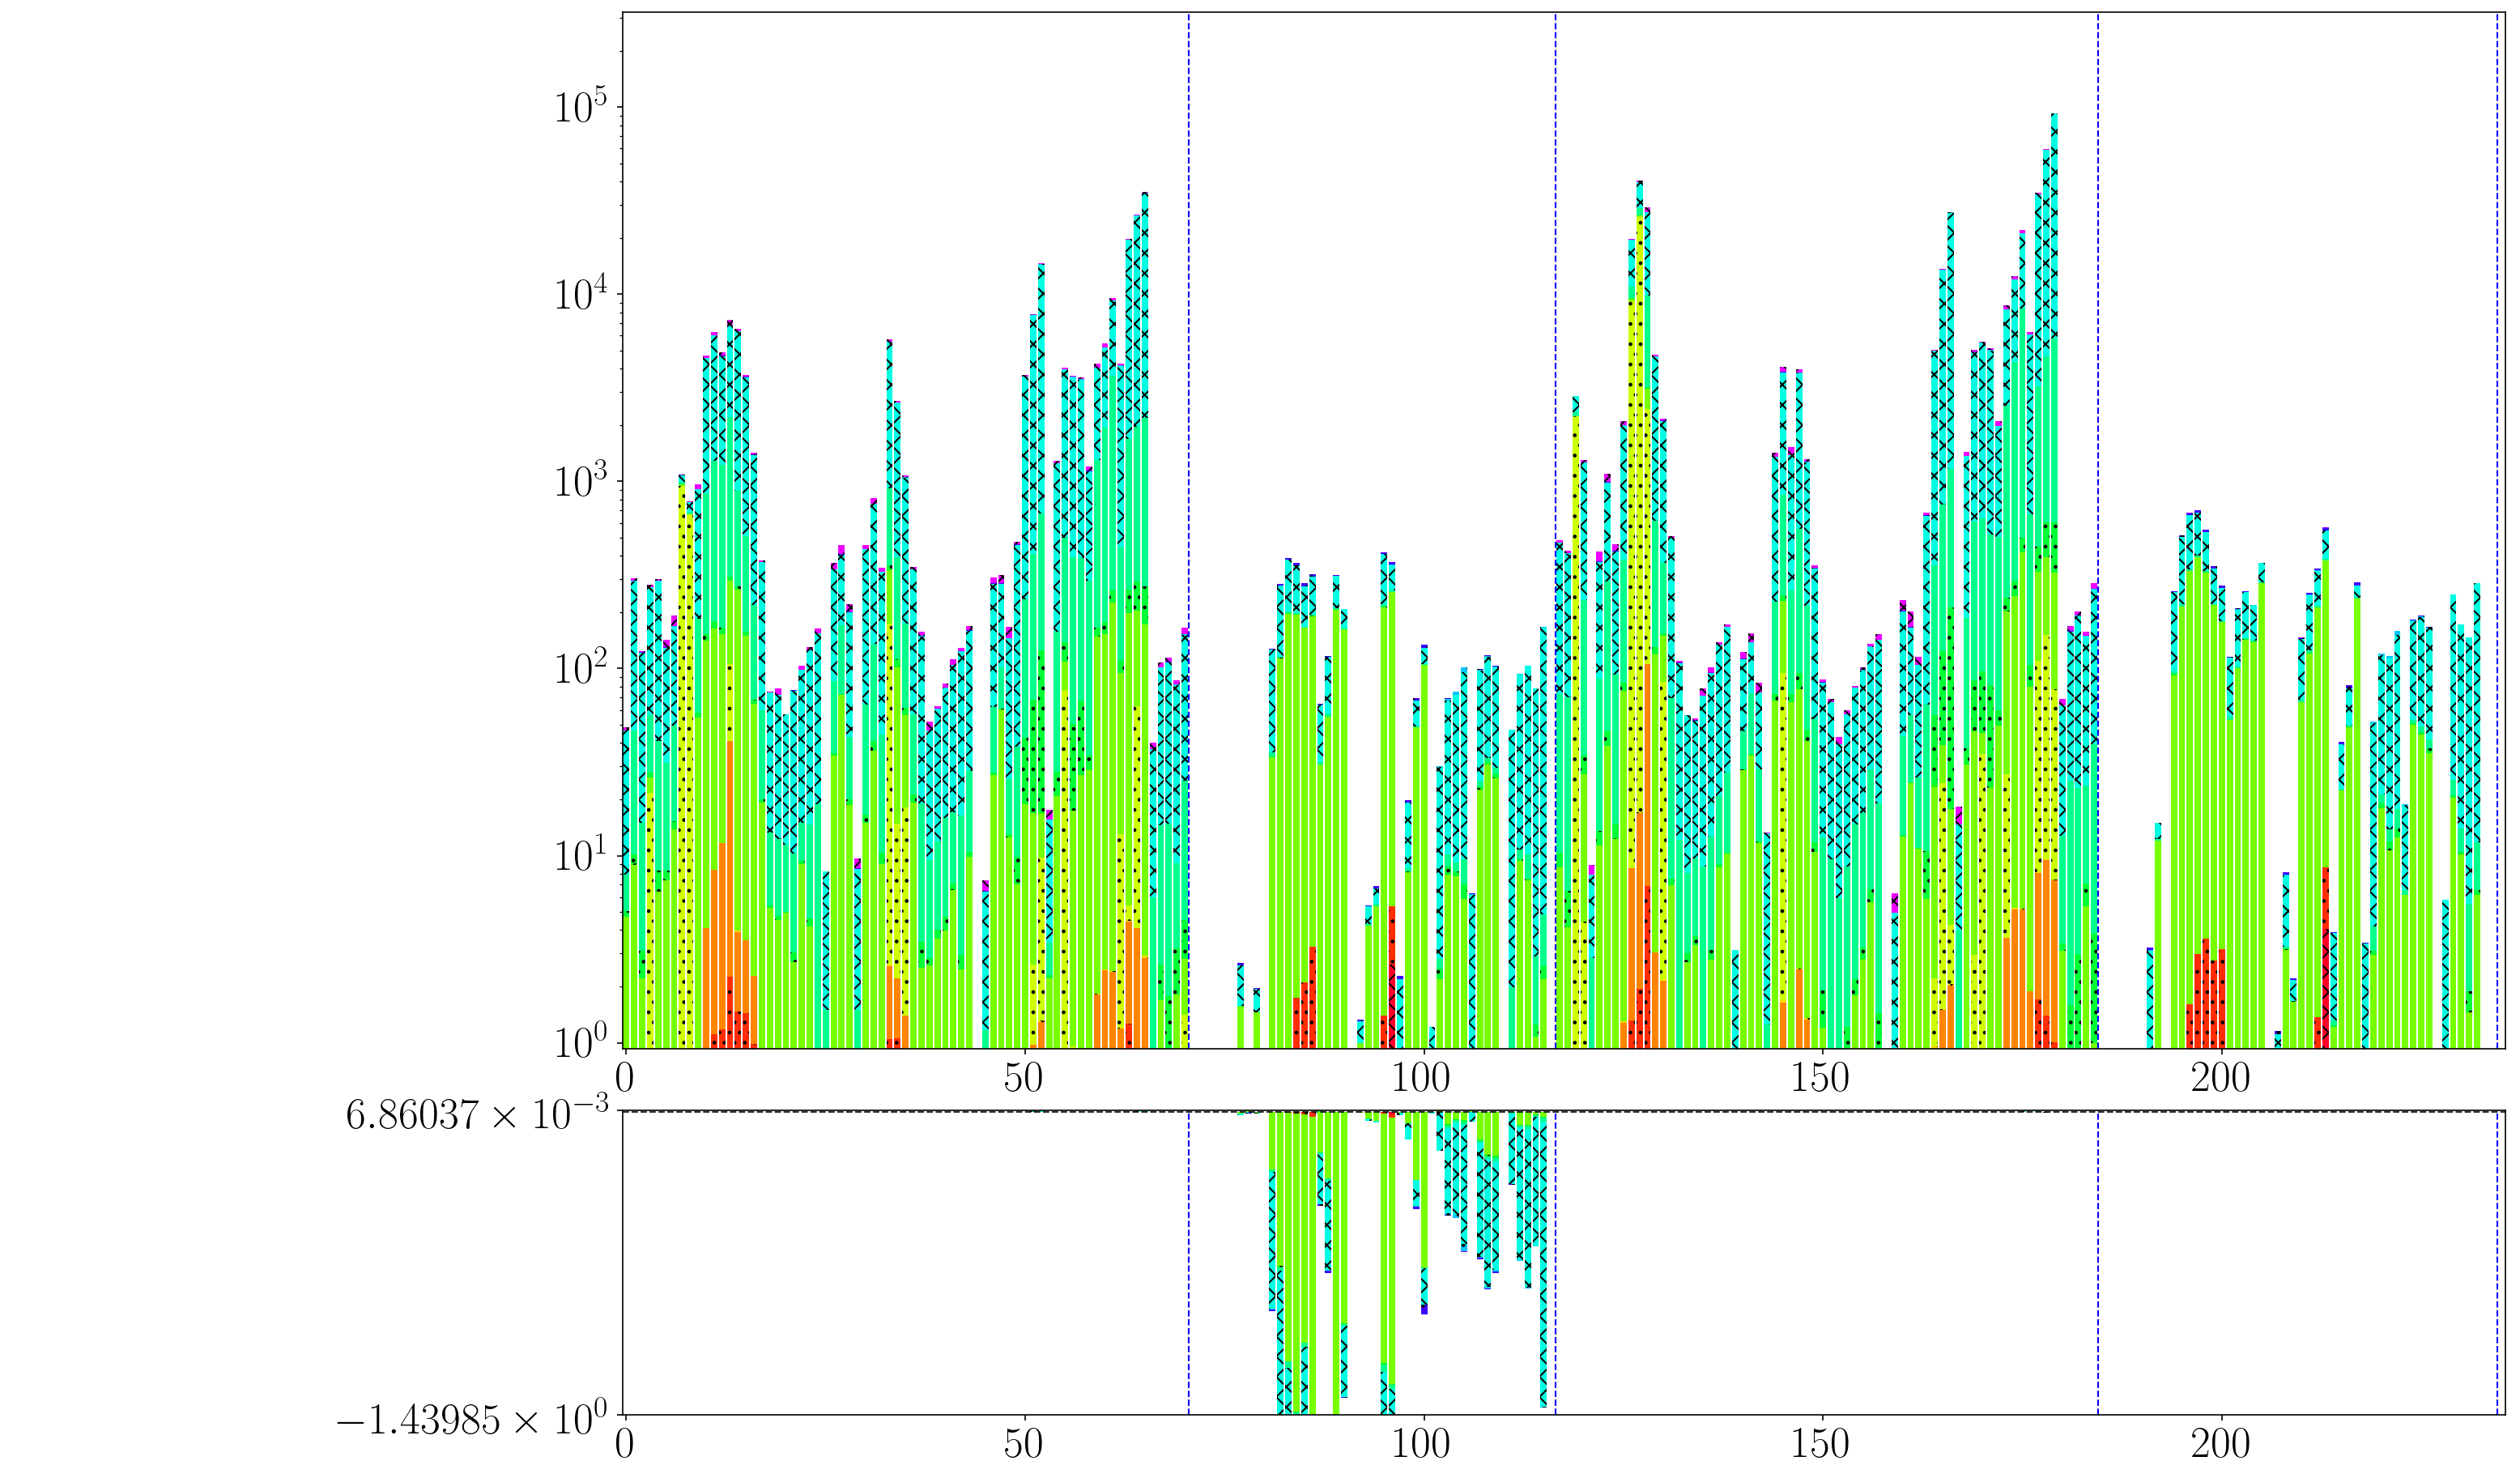
\includegraphics[width=\linewidth]{figures/network_setup/trigger_ee_sf_-0.5}
	\end{minipage}%
	\begin{minipage}{.5\textwidth}
		\centering
		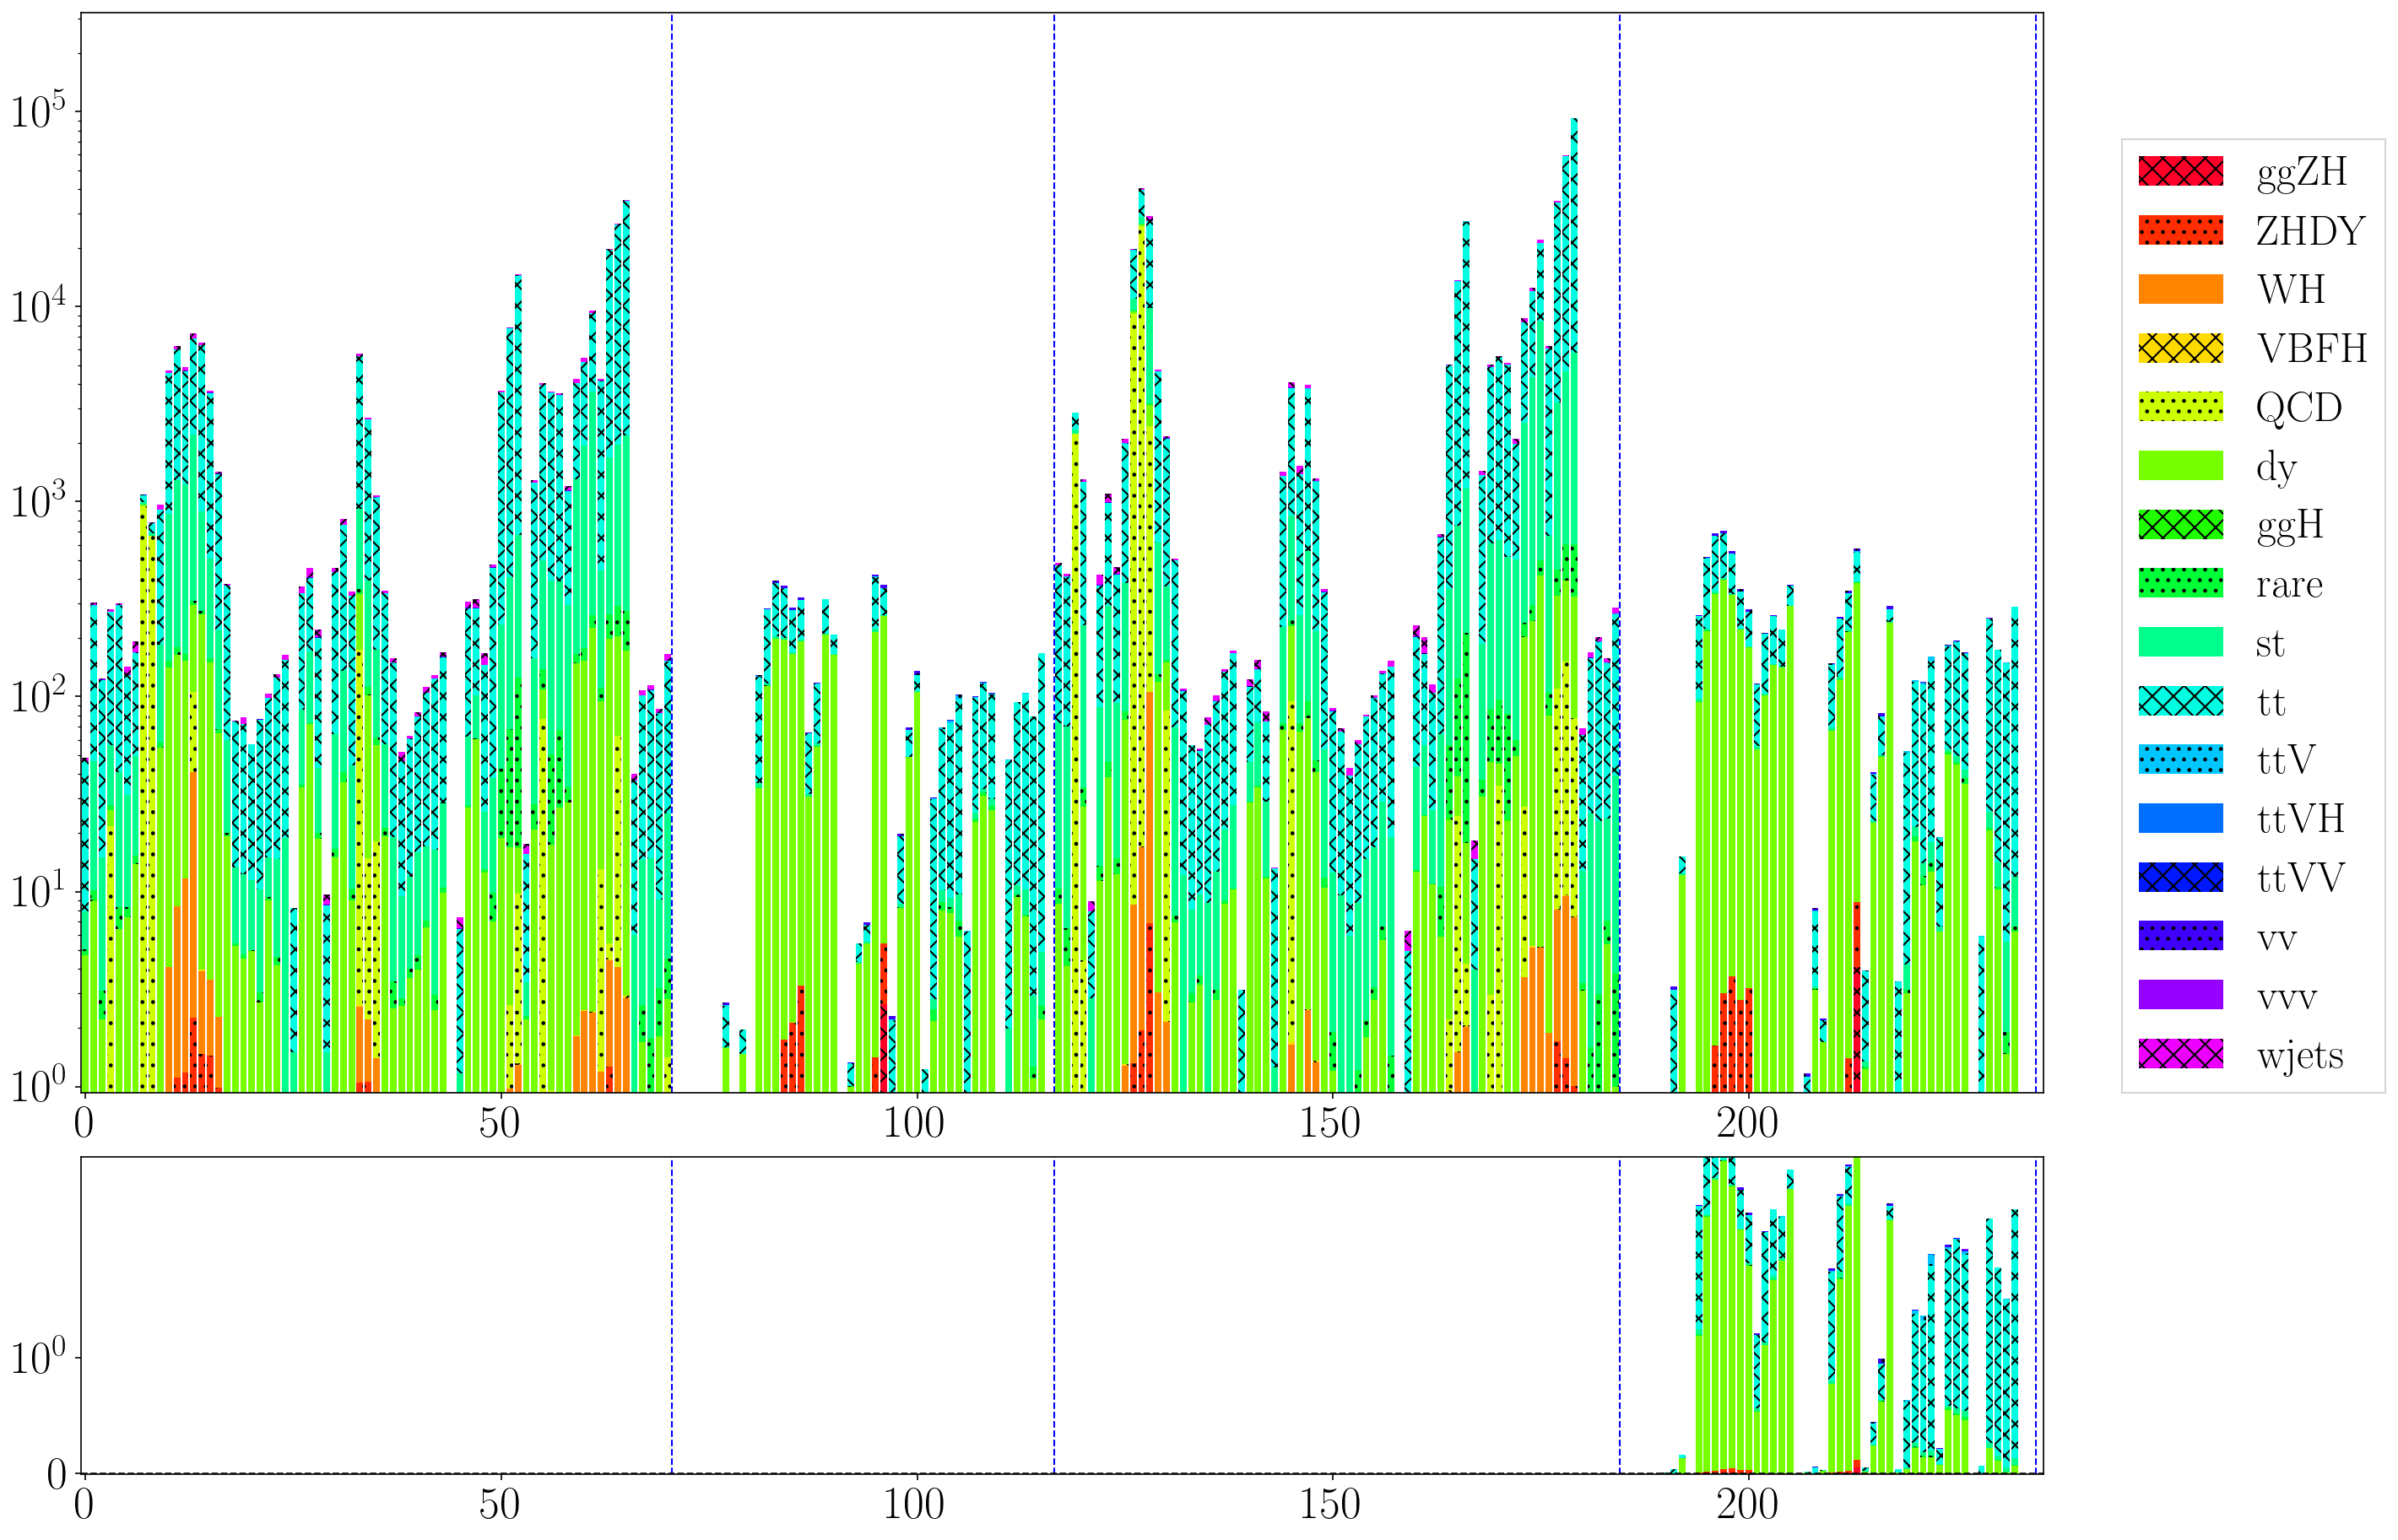
\includegraphics[width=\linewidth]{figures/network_setup/trigger_mumu_sf_+0.5}
		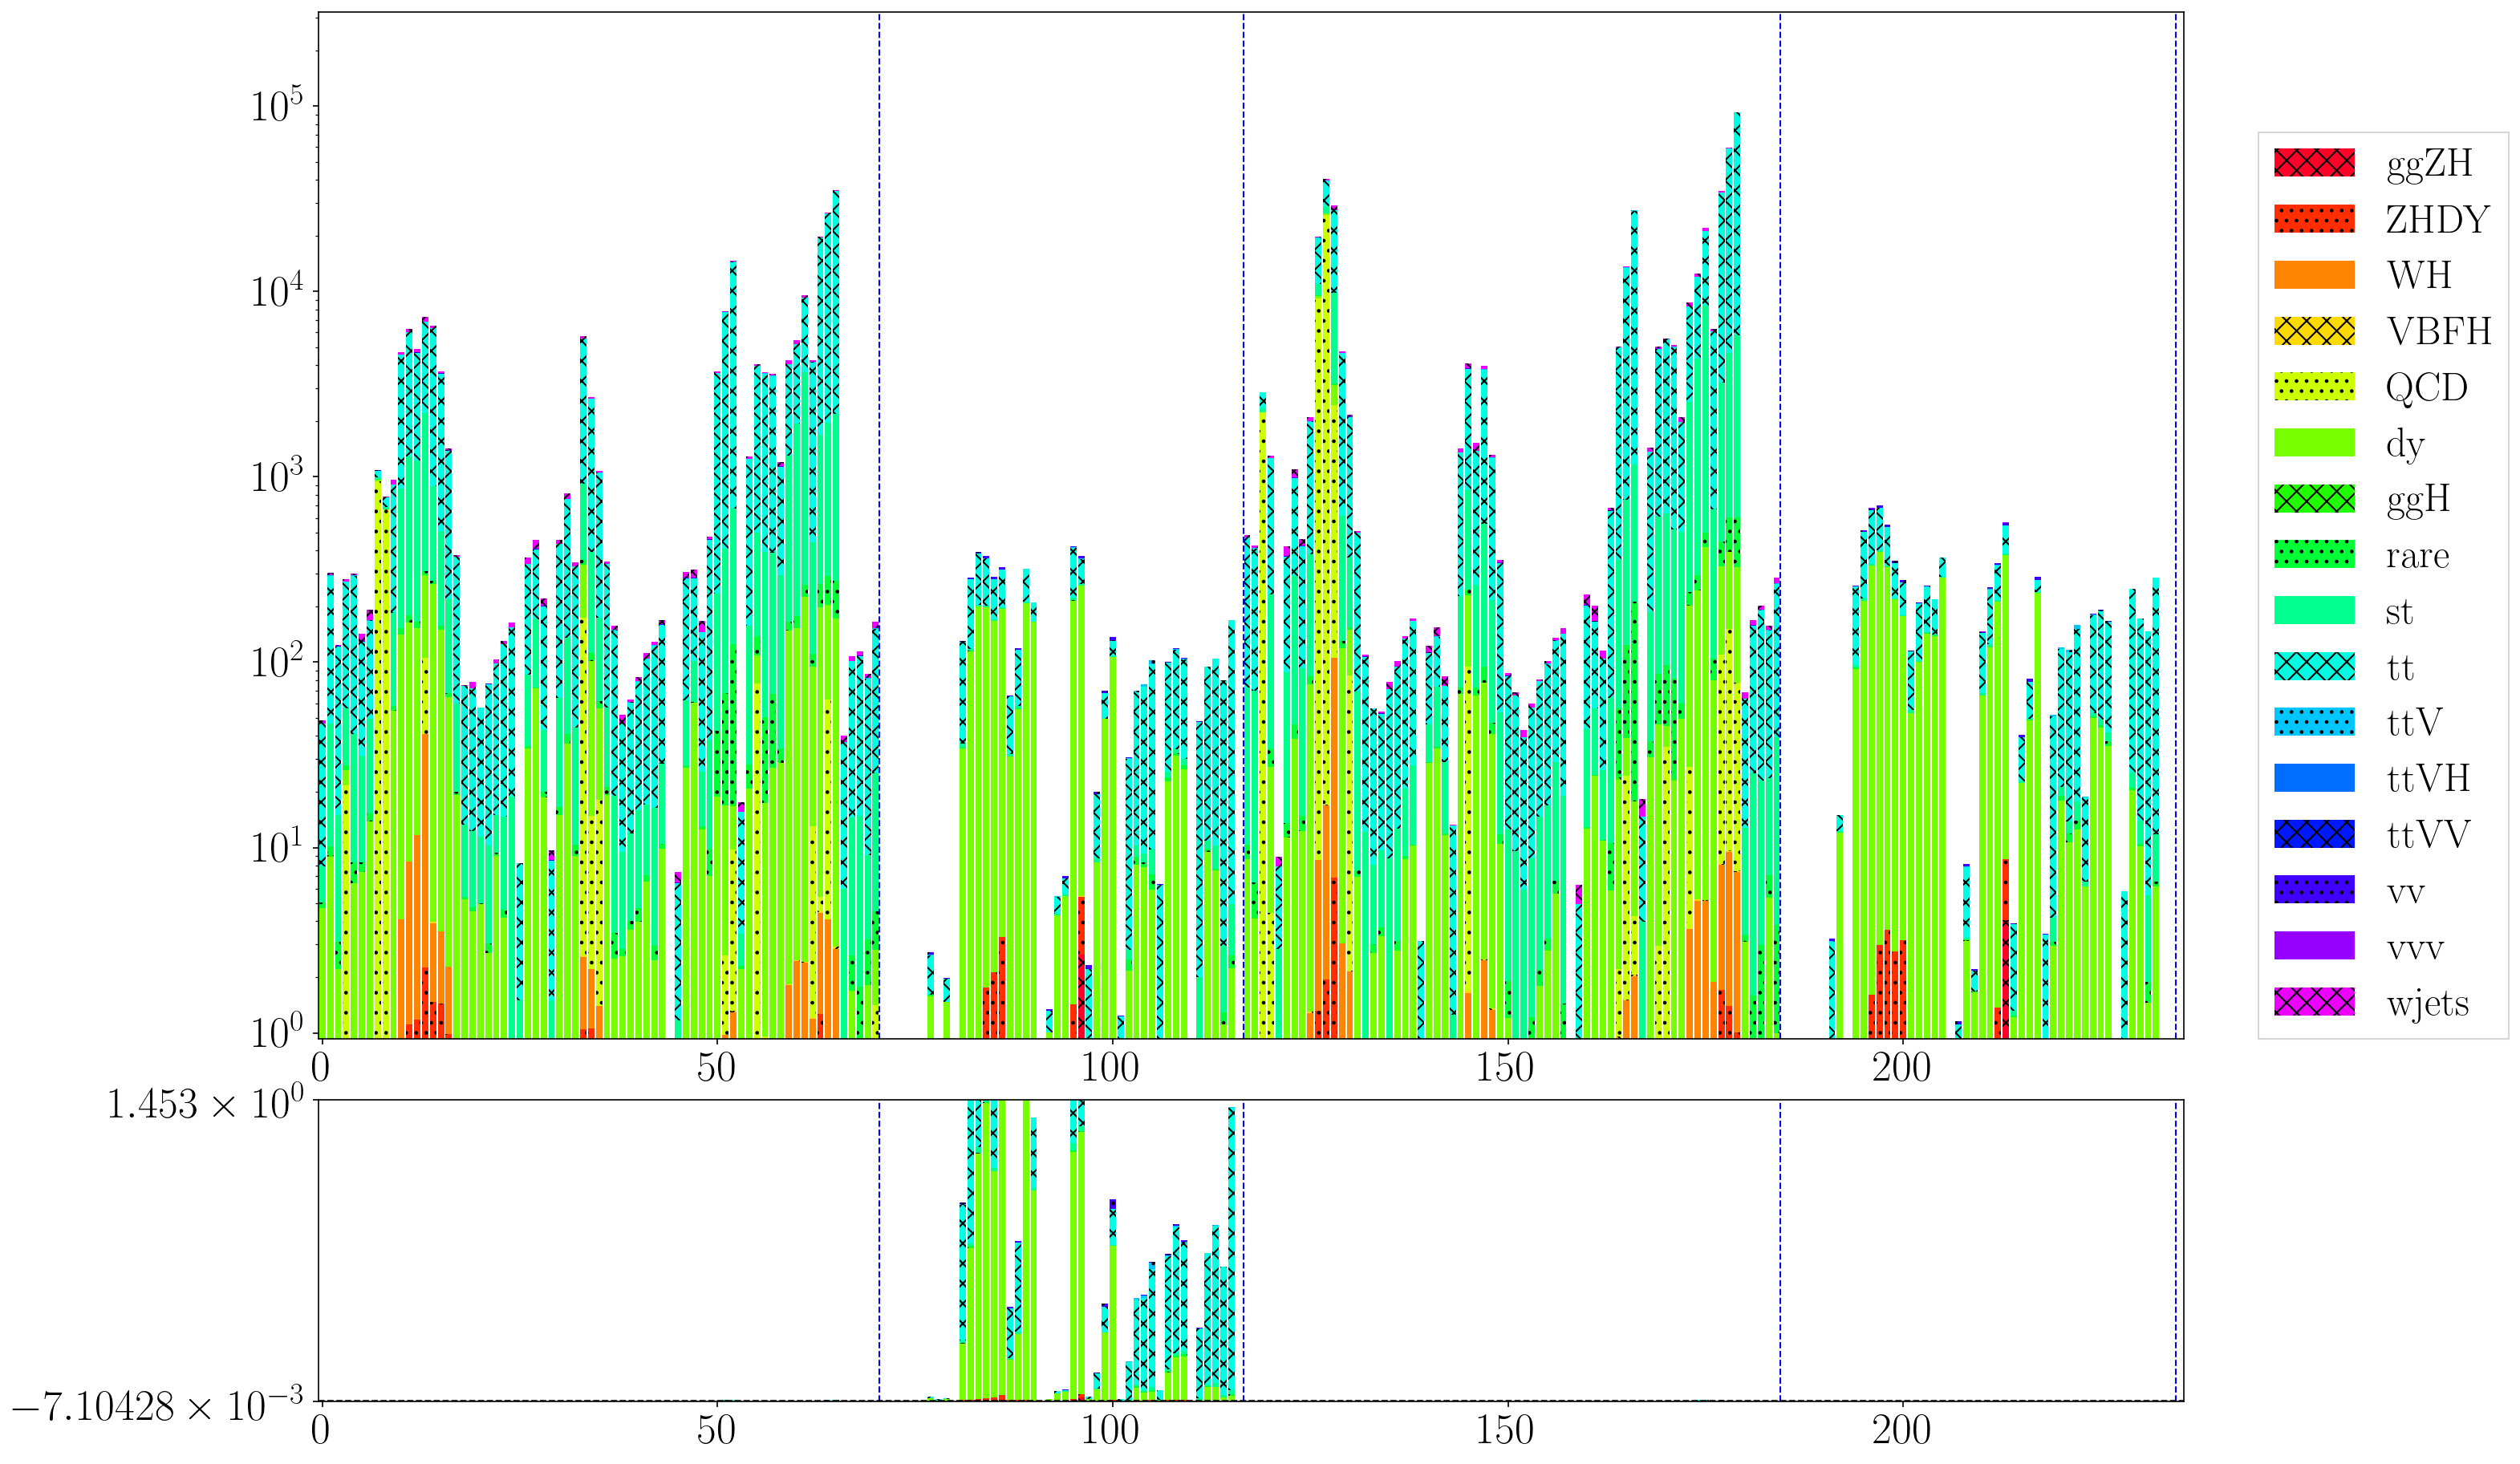
\includegraphics[width=\linewidth]{figures/network_setup/trigger_ee_sf_+0.5}
	\end{minipage}
	\caption{Morphed histograms for $m = -0.5$ (left) and $m = +0.5$ (right) for \texttt{trigger\_mumu\_sf} (above) and \texttt{trigger\_ee\_sf} (below). The four categories from left to right are: $e$, $ee$, $\mu$ and $\mu\mu$. Note the exclusive action of the efficiency uncertainties on a single category.}
	\label{fig:trigger_sf}
\end{figure}

\Subsection{\textcolor{red}{Statistical Uncertainties}}

There are two sources of statistical uncertainties on Monte Carlo level. First, there is a Poisson fluctuation due to the generator producing a finite amount of samples for each process. As the number of samples is large, one can assume that these fluctuations follow a normal distribution with $\mu = N$ and $\sigma = \sqrt{N}$. Second, it is expected that the data in the DNN-score histograms follow a Poisson distribution themselves.

The generator-related statistical effects have been applied following morphing, after which eventually arising negative values (due to the variation being performed through a normal distribution) have been clamped to zero. Then, the signal strength modifiers drawn from the prior distributions have been applied to each process and the resulting bins have been summed up, losing information on the exact bin content (just like in the case of real data). Last, the resulting histogram bin heights have been independently varied following a Poisson distribution to model statistical effects in the data and the application of the normalising luminosity uncertainty has been performed. The resulting histograms have been saved and used as training or test dataset.
\textcolor{red}{graph showing when to apply what effect?}

\Subsection{Network Architecture and Hyperparameters}

In the following, the cINN network architectures for the inference will be elaborated. The hyperparameters listed below have been systematically varied and those with the lowest test loss have been kept.

The network inputs are three signal and 13 background modifier parameter for each process and an additional normalizing nuisance parameter for the luminosity uncertainties. In total, the network has 17 inputs.

Regarding the conditions, it had a dimension of 235 for the four considered categories ($e$, $ee$, $\mu$ and $\mu\mu$) and all of their subcategories.

The implementation has been done in \texttt{Python} using \texttt{PyTorch} \cite{pytorch}; the network has been constructed using the "Framework for Easily Invertible Architectures" (\texttt{FrEIA}) framework \cite{freia}. The cINN uses 12 GLOW blocks. After each block, an additional permutation layer is introduced. These layers perform arbitrary (but fixed) permutations among the outputs. Note that this transformation has per construction a determinant of $\pm1$ making no change in the volume for the resulting normalizing flow. On the other hand, it does help removing any correlations between neighbouring input values, making training more performant.

The GLOW networks contain subnetworks with 128 Nodes, of 4 layers. The activation function for each layer was chosen to be ReLU.

For the summary network studies, a shallow network has been constructed, as more complex setups tended to overtrain in the considered cases. The network had a layer of 300 nodes between the DNN scores and the condition node; the output dimensionality has been chosen to be 100.

Both networks have been trained for 11000 epochs on the same dataset containing 1.5 million generated samples. For training, a batchsize of 500 has been chosen. For the test set, 150 000 samples have been generated.

The network inputs have been normalized to mean 0 and standard deviation 1 via

\begin{equation*}
	\mu^N_i = \frac{\mu_i - \langle\mu_i\rangle}{\sigma_{\mu_i}}
\end{equation*}

For the conditions, as they stretch over 5 orders of magnitude, their logarithm has been normalized:

\begin{equation*}
	y^N = \frac{\log(y+1)-\langle\log(y+1)\rangle}{\sigma_{\log(y+1)}}
\end{equation*}

As a learning rate scheduler, an empirically well-functioning cosine scheduler has been used. This scheduler starts off with a learning rate of $\eta = 10^{-3}$ and reduces it to $\eta = 10^{-5}$ in steps in each epoch. The evolution of the learning rate is shown in fig. \ref{fig:lr}. As an optimizer, Adam with parameters $\beta_1 = 0.9$ and $\beta_2 = 0.999$ has been chosen. In order to penalize large weights, a normalizing parameter of $\alpha = 10^{-5}$ has been chosen; for the clamping parameters, a value of 2 has been selected.

All tests have been performed three times (3 runs) with differently initialized models and the model with the lowest test loss has been studied further.

\begin{figure}[h!]
	\centering
	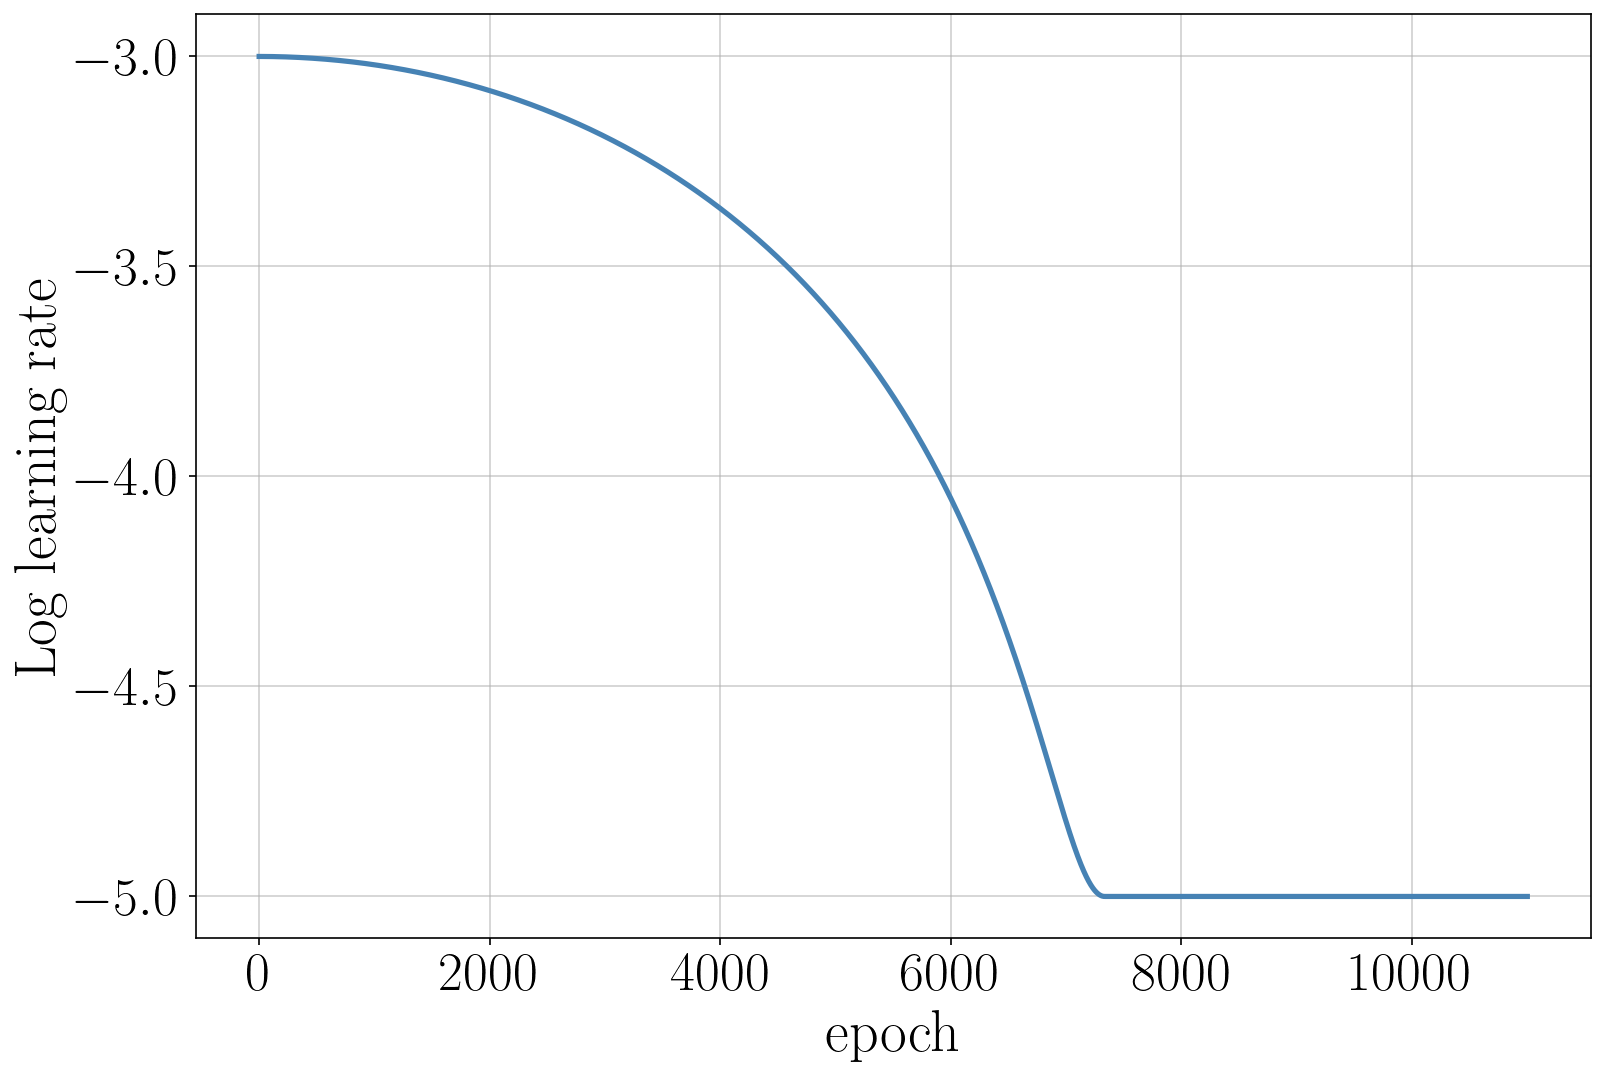
\includegraphics[width=0.6\linewidth]{figures/network_setup/lr}
	\caption{The evolution of the learning rate with each epoch on a logarithmic scale.}
	\label{fig:lr}
\end{figure}
